\documentclass[a4paper]{report}

\usepackage{../mathstemplate}

\date{IV семестр, весна 2024 г.}
\title{Алгебра. Неофициальный конспект}
\author{Лектор: Алексей Владимирович Степанов\\ Конспектировал Леонид Данилевич}

\begin{document}
    \shorthandoff{"}
    \maketitle
    \tableofcontents
    \newpage
    \setcounter{lection}{0}


    \chapter{Гомологическая алгебра}
    \newlection{12 февраля 2024 г.}
    \section{Абелевы категории}
    Напомним некоторые определения из предыдущей лекции.
    \definition[Предаддитивная категория $\cat{A}$]{
        $\forall A, B \in \cat{A}: \Mor_{\cat{A}}(A, B)$ образует абелеву группу, и везде, где определена, выполнена дистрибутивность: \[\alpha(\beta+\gamma) = \alpha\beta + \alpha\gamma \qquad (\beta + \gamma)\alpha = \beta\alpha + \gamma\alpha\]
    }
    \definition[Бипроизведение]{ Такая диаграмма, что
    % https://q.uiver.app/#q=WzAsMyxbMSwwLCJDIl0sWzAsMCwiQSJdLFsyLDAsIkIiXSxbMSwwLCJcXGlvdGFfMSIsMix7Im9mZnNldCI6MX1dLFswLDEsIlxccGlfMSIsMix7Im9mZnNldCI6MX1dLFswLDIsIlxccGlfMiIsMCx7Im9mZnNldCI6LTF9XSxbMiwwLCJcXGlvdGFfMiIsMCx7Im9mZnNldCI6LTF9XV0=
        \[\begin{tikzcd}[ampersand replacement=\&]
              A \& C \& B
              \arrow["{\iota_1}"', shift right, from=1-1, to=1-2]
              \arrow["{\pi_1}"', shift right, from=1-2, to=1-1]
              \arrow["{\pi_2}", shift left, from=1-2, to=1-3]
              \arrow["{\iota_2}", shift left, from=1-3, to=1-2]
        \end{tikzcd}\]
        \numbers{
            \item $\pi_1\iota_1 = \id_A$.
            \item $\pi_2\iota_2 = \id_B$.
            \item $ \iota_2 \pi_2+ \iota_1\pi_1  = \id_C$.
            \item $\pi_2\iota_1 = 0$.
            \item $\pi_1\iota_2 = 0$.
        }
    }
    \definition[Аддитивная категория]{
        Предаддитивная категория с финальным объектом и произведениями (любых двух объектов).
    }
    Эквивалентно, существуют инициальный объект и копроизведения, эквивалентно существуют нулевой объект и бипроизведения.
    \definition[Предабелева категория]{
        Аддитивная категория, в которой у всех морфизмов есть ядро и коядро.
    }
    \definition[(Ко)нормальный мономорфизм (эпиморфизм)]{
        Он является (ко)эквалайзером (какой-то, неважно какой, пары стрелок).
    }
    \definition[Абелева категория]{
        Предабелева категория, в которой все мономорфизмы нормальны.
    }
    Пусть $\cat C$ --- категория.
    Вспомним про категорию стрелок $\cat{Arr}\cat{C}$, в которой объекты --- стрелки из $\Mor(\cat C)$, множество морфизмов между $\phi, \psi$ --- это\[\Mor_{\cat{Arr}_{\cat{C}}}(\phi, \psi) = \defset{(\alpha, \beta)}{\alpha: \source(\phi) \map \source(\psi), \beta: \target(\phi) \map \target(\psi), \beta \phi = \psi \alpha}\]
    % https://q.uiver.app/#q=WzAsNCxbMCwwLCJcXGJ1bGxldCJdLFsxLDAsIlxcYnVsbGV0Il0sWzAsMSwiXFxidWxsZXQiXSxbMSwxLCJcXGJ1bGxldCJdLFswLDEsIlxccGhpIl0sWzIsMywiXFxwc2kiXSxbMCwyLCJcXGFscGhhIl0sWzEsMywiXFxiZXRhIl1d
    \[\begin{tikzcd}[ampersand replacement=\&]
          \bullet \& \bullet \\
          \bullet \& \bullet
          \arrow["\phi", from=1-1, to=1-2]
          \arrow["\psi", from=2-1, to=2-2]
          \arrow["\alpha", from=1-1, to=2-1]
          \arrow["\beta", from=1-2, to=2-2]
    \end{tikzcd}\]
    Далее будем обозначать за $\ker f$ ядро стрелки, как уравнитель стрелки и нуля, а за $\Ker f \coloneqq \source(\ker f)$ --- объект (в конкретных категориях типа $\modR{R}$ это докатегорное понятие ядра --- подмодуль без стрелки-вложения).
    \lemma{\label{ker-is-functor}
        $\ker, \coker$ --- функторы $\cat{Arr} \cat A \map \cat{Arr} \cat A$.
        \provehere{
            Достаточно доказать для ядер, для коядер двойственно.

        Определим действие $\ker$ на морфизмах:
        % https://q.uiver.app/#q=WzAsNixbMSwwLCJBIl0sWzEsMSwiQSciXSxbMiwwLCJCIl0sWzIsMSwiQiciXSxbMCwwLCJcXEtlciBmIl0sWzAsMSwiXFxLZXIgZiciXSxbMCwyLCJmIl0sWzEsMywiZiciXSxbMCwxLCJcXGFscGhhIl0sWzIsMywiXFxiZXRhIl0sWzQsMCwiXFxrZXIgZiJdLFs1LDEsIlxca2VyIGYnIl0sWzQsNSwiXFxleGlzdHMhXFxwaGkiLDAseyJsYWJlbF9wb3NpdGlvbiI6NDAsInN0eWxlIjp7ImJvZHkiOnsibmFtZSI6ImRhc2hlZCJ9fX1dXQ==
            \[\begin{tikzcd}[ampersand replacement=\&]
            {\Ker f} \& A \& B \\
            {\Ker f'} \& {A'} \& {B'}
            \arrow["f", from=1-2, to=1-3]
            \arrow["{f'}", from=2-2, to=2-3]
            \arrow["\alpha", from=1-2, to=2-2]
            \arrow["\beta", from=1-3, to=2-3]
            \arrow["{\ker f}", from=1-1, to=1-2]
            \arrow["{\ker f'}", from=2-1, to=2-2]
            \arrow["{\exists!\phi}"{pos=0.4}, dashed, from=1-1, to=2-1]
            \end{tikzcd}\]
            $f \cdot \ker f = 0 \then \beta \cdot f \cdot \ker f = 0 \then f' \cdot \alpha \cdot \ker f = 0$, откуда по универсальному свойству ядра $\exists !\phi: \ker f' \cdot \phi = \alpha \cdot \ker f$.

            Положим $\ker(\alpha, \beta) = (\phi, \alpha)$.
            Далее несложно проверить, что данное определение сохраняет композицию и $\id$.
        }
    }
    \definition[Точный функтор]{Функтор, сохраняющий ядра и коядра.}
    \intfact[Теорема Фрейда --- Митчелла (Freyd --- Mitchell)] {\label{mitchell}
    Для любой малой абелевой категории $\cat{A}$: $\exists R \in \cat{Ring}$ (необязательно коммутативное кольцо с единицей) и строгий, полный, точный функтор $\cat{A} \map \modR{R}$.
    }
    \proposal{
        Для всякого морфизма $f: A \map B$ найдётся пунктирная стрелка, делающая диаграмму коммутативной.
% https://q.uiver.app/#q=WzAsNixbMCwwLCJcXEtlciBmIl0sWzEsMCwiQSJdLFsyLDAsIkIiXSxbMywwLCJcXENvS2VyIGYiXSxbMSwxLCJcXENvS2VyIFxca2VyIGYiXSxbMiwxLCJcXEtlciBcXGNva2VyIGYiXSxbMSwyLCJmIl0sWzAsMSwiXFxrZXIgZiJdLFsyLDMsIlxcY29rZXIgZiJdLFsxLDQsIlxcY29rZXJcXGtlciBmIiwyXSxbNSwyLCJcXGtlciBcXGNva2VyIGYiLDJdLFs0LDUsIlxcZXhpc3RzISIsMCx7InN0eWxlIjp7ImJvZHkiOnsibmFtZSI6ImRhc2hlZCJ9fX1dXQ==
        \[\begin{tikzcd}[ampersand replacement=\&]
        {\Ker f} \& A \& B \& {\CoKer f} \\
        \& {\CoKer \ker f} \& {\Ker \coker f}
        \arrow["f", from=1-2, to=1-3]
        \arrow["{\ker f}", from=1-1, to=1-2]
        \arrow["{\coker f}", from=1-3, to=1-4]
        \arrow["{\coker\ker f}"', from=1-2, to=2-2]
        \arrow["{\ker \coker f}"', from=2-3, to=1-3]
        \arrow["{\exists!}", dashed, from=2-2, to=2-3]
        \end{tikzcd}\]
        Более того, в абелевой категории эта стрелка --- изоморфизм.
        \provehere{
            Следует из эпи-моно разложения, доказанного на прошлой лекции, или из теоремы Митчелла.

            Само построение пунктирной стрелки получается из универсальных свойств, а доказательство того, что это --- изо --- непростое.
        }
    }
    \lemma{\label{when-ab} Пусть $\cat C$ --- полная подкатегория в абелевой категории $\cat A$. Следующие условия равносильны
    \bullets{
        \item $\cat C$ является абелевой.
        \item \bullets{
            \item $0_{\cat A} \in \cat C$, здесь, как обычно, $0_{\cat A}$ --- нулевой объект категории $\cat A$.
            \item $\cat C$ содержит бипроизведение любых двух своих объектов.
            \item Ядра и коядра (взятые в $\cat A$) любых морфизмов из $\cat C$ лежат в $\cat C$.
        }
    }
    \provewthen{
        Очевидно.
    }{
        Чуть сложнее, доказывать не будем (и использовать тоже).
    }
    }
    \section{Компл$\acute{\text{е}}$ксы}
    Если противное не оговорено, то всё происходит в абелевой категории $\cat A$, большими буквами обозначены объекты данной категории, маленькими --- морфизмы.
    \definition[Компл$\acute{\text{е}}$кс]{
        Такая диаграмма, что $\forall k \in \Z: d_k \cdot d_{k+1} = 0$.
        % https://q.uiver.app/#q=WzAsNSxbMSwwLCJDX3tuKzF9Il0sWzIsMCwiQ19uIl0sWzMsMCwiQ197bi0xfSJdLFswLDAsIlxcY2RvdHMiXSxbNCwwLCJcXGNkb3RzIl0sWzMsMCwiZF97bisxfSJdLFswLDEsImRfbiJdLFsxLDIsImRfe24tMX0iXSxbMiw0LCJkX3tuLTJ9Il1d
        \[\begin{tikzcd}[ampersand replacement=\&]
              \cdots \& {C_{n+1}} \& {C_n} \& {C_{n-1}} \& \cdots
              \arrow["{d_{n+1}}", from=1-1, to=1-2]
              \arrow["{d_n}", from=1-2, to=1-3]
              \arrow["{d_{n-1}}", from=1-3, to=1-4]
              \arrow["{d_{n-2}}", from=1-4, to=1-5]
        \end{tikzcd}\]
    }
    Альтернативно, комплекс можно рассматривать, как функтор из категории $(\Z, \ge)$ (полученной из частично упорядоченного множества) в $\cat A$ (при котором образ композиции любых двух нетождественных морфизмов нулевой).
    Таким образом, комплексы --- полная подкатегория в категории этих функторов.

    Ещё один, следующий, взгляд на комплексы работает только для конкретной категории, уже вложенной в $R$-модули.
    \definition[Градуированный объект]{
        $C_{\bullet} = \bigoplus\limits_{n \in \Z}C_n$ с морфизмом $d: C_\bullet \map C_\bullet$, таким, что $d(C_n) \subset C_{n+p}$ для некоторой фиксированной \emph{степени объекта} $p$ (чаще всего она равна $\pm1$).
    }
    \definition[Дифференциальный модуль]{
        Градуированный объект $(C_\bullet, d)$ со свойством $d^2 = 0$.
    }
    \definition[Комплекс]{ Дифференциальный модуль степени $-1$. }
    При развороте стрелок получается дифференциальный модуль степени $+1$, также известный, как \emph{кокомплекс}:
    % https://q.uiver.app/#q=WzAsNSxbMCwwLCJcXGNkb3RzIl0sWzEsMCwiQ157bisxfSJdLFsyLDAsIkNee259Il0sWzMsMCwiQ157bi0xfSJdLFs0LDAsIlxcY2RvdHMiXSxbMSwwLCJkXntuKzJ9IiwyXSxbMiwxLCJkXntuKzF9IiwyXSxbMywyLCJkXm4iLDJdLFs0LDMsImRee24tMX0iLDJdXQ==
    \[\begin{tikzcd}[ampersand replacement=\&]
          \cdots \& {C^{n+1}} \& {C^{n}} \& {C^{n-1}} \& \cdots
          \arrow["{d^{n+2}}"', from=1-2, to=1-1]
          \arrow["{d^{n+1}}"', from=1-3, to=1-2]
          \arrow["{d^n}"', from=1-4, to=1-3]
          \arrow["{d^{n-1}}"', from=1-5, to=1-4]
    \end{tikzcd}\]
    \precaution{
    У кокомплекса несколько другая нумерация стрелок, но мы их практически не будем использовать.
    }
    \definition[Сдвиг комплекса $(C_\bullet, d)$ на $p \in \Z$]{
        Комплекс $(C[p]_\bullet, d[p])$, где $C[p]_n = C_{n+p}$ и $d[p]_n = d_{n+p}$.
    }
    Иногда при сдвиге комплекса определяют $d[p]_n = (-1)^p d_{n+p}$, но мы так делать не будем.
    \newlection{19 февраля 2023 г.}
    \definition[Морфизм дифференциальных модулей $\bigoplus A_n \map \bigoplus B_n$]{
        Такое $f: \bigoplus A_n \map \bigoplus B_n$, что $f(A_n) \subset B_n$, и диаграммы коммутативны:
        % https://q.uiver.app/#q=WzAsNCxbMCwwLCJBX3tuKzF9Il0sWzEsMCwiQV9uIl0sWzAsMSwiQl97bisxfSJdLFsxLDEsIkJfbiJdLFswLDEsImRfbl5BIl0sWzIsMywiZF9uXkIiXSxbMCwyLCJmIl0sWzEsMywiZiJdXQ==
        \[\begin{tikzcd}[ampersand replacement=\&]
        {A_{n+1}} \& {A_n} \\
        {B_{n+1}} \& {B_n}
        \arrow["{d_n^A}", from=1-1, to=1-2]
        \arrow["{d_n^B}", from=2-1, to=2-2]
        \arrow["f", from=1-1, to=2-1]
        \arrow["f", from=1-2, to=2-2]
        \end{tikzcd}\]
        На языке абелевых категорий, надо рассматривать не одно отображение $f$, так как отношение $f(A_n) \subset B_n$ не выражается, а серию морфизмов $f_n: A_n \map B_n$.
    }
    Для всякого морфизма $f$ коммутативна диаграмма в категории комплексов:
    % https://q.uiver.app/#q=WzAsNCxbMCwwLCJBWzFdIl0sWzEsMCwiQSJdLFswLDEsIkJbMV0iXSxbMSwxLCJCIl0sWzAsMSwiZF5BIl0sWzIsMywiZF5CIl0sWzAsMiwiZlsxXSJdLFsxLDMsImYiXV0=
    \[\begin{tikzcd}[ampersand replacement=\&]
    {A[1]} \& A \\
    {B[1]} \& B
    \arrow["{d^A}", from=1-1, to=1-2]
    \arrow["{d^B}", from=2-1, to=2-2]
    \arrow["{f[1]}", from=1-1, to=2-1]
    \arrow["f", from=1-2, to=2-2]
    \end{tikzcd}\]
    Если рассматривать комплексы, как функторы из категории $(\Z, \ge)$, то морфизмы между комплексами --- естественные преобразования между функторами.
    \theorem{
    Категория комплексов абелева.
    \provehere{
    \indentlemma{
        Если $\cat C$ --- малая категория, $\cat A$ --- абелева, то $\Func(\cat C, \cat A)$ --- тоже абелева категория.
    }{
        Нулевой объект --- функтор $\0$, сопоставляющий каждому объекту $0_{\cat A}$, и каждой стрелке --- нуль-стрелку.

        Для двух функторов $\cat F, \cat G$: $(\cat F \oplus \cat G)(C) = \cat F(C) \oplus \cat G(C)$.

        Если $\eta \in \Mor_{\Func(\cat C, \cat A)}(\cat F, \cat G)$ (то есть $\eta$ --- естественное преобразование $\cat F \map \cat G$), то $(\Ker \eta)(C) = \Ker (\eta_C)$.

        Аналогично~(\cref{ker-is-functor}), определяется $\ker$. Аналогично с коядрами.

        Далее по-хорошему надо проверить, что выполняются все универсальные свойства, но мы этого делать не будем.
    }
    Ссылаемся на~(\cref{when-ab}).
    % https://q.uiver.app/#q=WzAsMTUsWzEsMCwiQV97bisxfSJdLFsyLDAsIkFfbiJdLFszLDAsIkFfe24tMX0iXSxbMCwwLCJcXGNkb3RzIl0sWzQsMCwiXFxjZG90cyJdLFswLDEsIlxcY2RvdHMiXSxbMSwxLCJCX3tuKzF9Il0sWzIsMSwiQl9uIl0sWzMsMSwiQl97bi0xfSJdLFs0LDEsIlxcY2RvdHMiXSxbMSwyLCJBX3tuKzF9XFxvcGx1cyBCX3tuKzF9Il0sWzIsMiwiQV9uIFxcb3BsdXMgQl9uIl0sWzMsMiwiQV97bi0xfSBcXG9wbHVzIEJfe24tMX0iXSxbMCwyLCJcXGNkb3RzIl0sWzQsMiwiXFxjZG90cyJdLFszLDBdLFswLDEsImReQV9uIl0sWzEsMiwiZF5BX3tuLTF9Il0sWzIsNF0sWzUsNl0sWzYsNywiZF5CX24iXSxbNyw4LCJkXkJfe24tMX0iXSxbOCw5XSxbMTAsMTEsImRee0EgXFxvcGx1cyBCfV9uIl0sWzExLDEyLCJkXntBIFxcb3BsdXMgQn1fe24tMX0iXSxbMTMsMTBdLFsxMiwxNF1d
        \[\begin{tikzcd}[ampersand replacement=\&]
              \cdots \& {A_{n+1}} \& {A_n} \& {A_{n-1}} \& \cdots \\
              \cdots \& {B_{n+1}} \& {B_n} \& {B_{n-1}} \& \cdots \\
              \cdots \& {A_{n+1}\oplus B_{n+1}} \& {A_n \oplus B_n} \& {A_{n-1} \oplus B_{n-1}} \& \cdots
              \arrow[from=1-1, to=1-2]
              \arrow["{d^A_n}", from=1-2, to=1-3]
              \arrow["{d^A_{n-1}}", from=1-3, to=1-4]
              \arrow[from=1-4, to=1-5]
              \arrow[from=2-1, to=2-2]
              \arrow["{d^B_n}", from=2-2, to=2-3]
              \arrow["{d^B_{n-1}}", from=2-3, to=2-4]
              \arrow[from=2-4, to=2-5]
              \arrow["{d^{A \oplus B}_n}", from=3-2, to=3-3]
              \arrow["{d^{A \oplus B}_{n-1}}", from=3-3, to=3-4]
              \arrow[from=3-1, to=3-2]
              \arrow[from=3-4, to=3-5]
        \end{tikzcd}\]
    Если $d^A \cdot d^A = 0$, и $d^B \cdot d^B = 0$, то (из теоремы Митчелла уж точно очевидно) $d^{A \oplus B} \cdot d^{A \oplus B} = 0$.

    Ядра тоже являются комплексами, так как на языке конкретных категорий это просто подмодули.
        Двойственно с коядрами.
    }
    }
    \section{Гомологии}
    Дифференциал $d$ является морфизмом комплексов $d: C[1] \map C$ (по-хорошему, $C[1]_\bullet \map C_\bullet$, но точку будем опускать):
    % https://q.uiver.app/#q=WzAsOCxbMCwwLCJcXGNkb3RzIl0sWzEsMCwiQ197bisxfSJdLFsyLDAsIkNfbiJdLFszLDAsIlxcY2RvdHMiXSxbMCwxLCJcXGNkb3RzIl0sWzEsMSwiQ19uIl0sWzIsMSwiQ197bi0xfSJdLFszLDEsIlxcY2RvdHMiXSxbMCwxXSxbMSwyLCJkX24iXSxbMiwzXSxbNiw3XSxbNSw2LCJkX3tuLTF9Il0sWzQsNV0sWzEsNSwiZF9uIl0sWzIsNiwiZF97bi0xfSJdXQ==
    \[\begin{tikzcd}[ampersand replacement=\&]
          \cdots \& {C_{n+1}} \& {C_n} \& \cdots \\
          \cdots \& {C_n} \& {C_{n-1}} \& \cdots
          \arrow[from=1-1, to=1-2]
          \arrow["{d_n}", from=1-2, to=1-3]
          \arrow[from=1-3, to=1-4]
          \arrow[from=2-3, to=2-4]
          \arrow["{d_{n-1}}", from=2-2, to=2-3]
          \arrow[from=2-1, to=2-2]
          \arrow["{d_n}", from=1-2, to=2-2]
          \arrow["{d_{n-1}}", from=1-3, to=2-3]
    \end{tikzcd}\]
    Ниже мы по произвольному комплексу $C$ строим новые комплексы.
    \definition[Циклы]{Комплекс $Z = Z(C) \bydef \Ker d[-1]$.}
    \definition[Границы]{Комплекс $B = B(C) \bydef \Image d[-1]$.}
    По определению, образ --- это ядро коядра: $\Image \phi \bydef \Ker(\coker \phi)$.
    В абелевой категории канонически $\Image \phi \cong \CoIm \phi \bydef \CoKer(\ker \phi)$.

    На языке конкретных категорий, так как $d^2 = 0$, то $B \subset Z$, и можно определить фактормодуль $H \coloneqq Z/B$ --- \emph{гомологии}.

    То же самое можно сказать на языке универсальных свойств, хотя в будущем мы, ссылаясь на теорему Митчелла, будем всё писать исключительно в терминах элементов.
    % https://q.uiver.app/#q=WzAsOCxbMCwwLCJaWzFdIl0sWzEsMCwiQ1sxXSJdLFsxLDEsIkIiXSxbMiwwLCJDIl0sWzMsMCwiQ1stMV0iXSxbMiwxLCJaIl0sWzMsMSwiSCJdLFs0LDEsIjAiXSxbMyw0LCJkWy0xXSJdLFsxLDMsImQiXSxbMSwyLCJiIiwyXSxbMCwxLCJ6WzFdIl0sWzUsMywieiIsMl0sWzEsNSwiXFxhbHBoYSIsMSx7InN0eWxlIjp7ImJvZHkiOnsibmFtZSI6ImRhc2hlZCJ9fX1dLFsyLDUsIlxcYmV0YSIsMix7InN0eWxlIjp7ImJvZHkiOnsibmFtZSI6ImRvdHRlZCJ9fX1dLFs1LDYsIlxcY29rZXJcXGJldGEiLDIseyJzdHlsZSI6eyJib2R5Ijp7Im5hbWUiOiJkb3R0ZWQifX19XSxbNiw3LCIiLDAseyJzdHlsZSI6eyJib2R5Ijp7Im5hbWUiOiJkb3R0ZWQifX19XV0=
    \[\begin{tikzcd}[ampersand replacement=\&]
    {Z[1]} \& {C[1]} \& C \& {C[-1]} \\
    \& B \& Z \& H \& 0
    \arrow["{d[-1]}", from=1-3, to=1-4]
    \arrow["d", from=1-2, to=1-3]
    \arrow["b"', from=1-2, to=2-2]
    \arrow["{z[1]}", from=1-1, to=1-2]
    \arrow["z"', from=2-3, to=1-3]
    \arrow["\alpha"{description}, dashed, from=1-2, to=2-3]
    \arrow["\beta"', dotted, from=2-2, to=2-3]
    \arrow["\coker\beta"', dotted, from=2-3, to=2-4]
    \arrow[dotted, from=2-4, to=2-5]
    \end{tikzcd}\]
    \provehere[Построение $H$ в терминах универсальных свойств]{
        Так как $d[-1] \cdot d = 0$, то можно пропуститься через ядро: $\exists! \alpha: z \cdot \alpha = d$.

    Далее, $z \cdot \alpha \cdot z[1] = d \cdot z[1] = 0$, а так как $z$ --- моно, то $\alpha \cdot z[1] = 0$.
    Значит, можно пропуститься через коядро, то есть $\exists ! \beta: \beta b = \alpha$.
    Далее $H$ определяется, как коядро $\beta$.
    }
    \corollary{
        В комплексах $Z, B, H$ нулевые дифференциалы.
        \provehere{
            Из диаграммы следует, что в комплексе $Z$ нулевые дифференциалы.
            $B$ состоит из подмодулей в $Z$, $H$ --- из фактормодулей, понятно, что там дифференциалы тоже нулевые.
        }
    }
    \examples[Гомологии окружности]{
        \item Рассмотрим окружность, как симплициальное множество:
        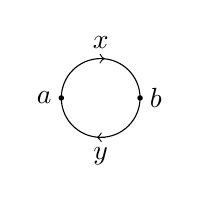
\begin{tikzpicture}[baseline=-4]
            \draw(0,0) circle[radius=0.5];
            \fill (-0.5,0) circle (1pt) node[left] {$a$};
            \fill (0.5,0) circle (1pt) node[right] {$b$};
            \node[above] at (0, 0.5) {$x$};
            \node[below] at (0, -0.5) {$y$};
            \draw[->] (-0.05, 0.5) -- (0.05, 0.5);
            \draw[<-] (-0.05, -0.5) -- (0.05, -0.5);
        \end{tikzpicture}

    Построим $C_0 = \Z a + \Z b$ --- свободная абелева группа на $\{a, b\}$, $C_1 = \Z x + \Z y$ --- тоже свободная абелева группа, но на образующих $\{x, y\}$.
        Вместо $\Z$ можно было взять любое другое кольцо.

    Все остальные элементы комплекса объявляются нулями.
    % https://q.uiver.app/#q=WzAsNCxbMCwwLCIwIl0sWzEsMCwiQ18xIl0sWzIsMCwiQ18wIl0sWzMsMCwiMCJdLFsyLDNdLFsxLDIsImRfMSJdLFswLDFdXQ==
        \[\begin{tikzcd}[ampersand replacement=\&]
              0 \& {C_1} \& {C_0} \& 0
              \arrow[from=1-3, to=1-4]
              \arrow["{d_1}", from=1-2, to=1-3]
              \arrow[from=1-1, to=1-2]
        \end{tikzcd}\]

    Определим $d_1$, как <<конец минус начало>>: $\all{d_1(x) = b - a,\\ d_1(y) = a - b}$.

    Теперь $\all{Z_0 = C_0 \\ Z_1 = \Z(x + y)} \all{B_0 = \Z(b - a) \\ B_1 = 0}$ и $\all{H_0 = Z_0 / B_0 = (\Z a + \Z b)/\Z(b - a) &\cong \Z \\ H_1 = Z_1/B_1 = \Z(x + y) &\cong \Z}$.
    \item Теперь триангулируем окружность по-другому:
        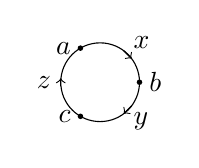
\begin{tikzpicture}[baseline=-4]
            \draw(0,0) circle[radius=0.5];
            \fill (-0.25,0.433) circle (1pt) node[left] {$a$};
            \fill (-0.25,-0.433) circle (1pt) node[left] {$c$};
            \fill (0.5,0) circle (1pt) node[right] {$b$};
            \node[above,right] at (0.3, 0.5) {$x$};
            \node[below,right] at (0.3, -0.5) {$y$};
            \node[left] at (-0.5, 0) {$z$};
            \draw[->] (-0.5, -0.05) -- (-0.5, 0.05);
            \draw[->] (0.3, 0.4) -- (0.4, 0.3);
            \draw[->] (0.4, -0.3) -- (0.3, -0.4);
        \end{tikzpicture}
    $\all{d_1(x) = b - a,\\ d_1(y) = c - b,\\ d_1(z) =  a - c}$.

    Теперь $\all{Z_0 = C_0 \\ Z_1 = \Z(x + y + z)}$, $\all{B_0 = \Z(b - a) + \Z(c - b) \\ B_1 = 0}$ и $\all{H_0  &\cong \Z \\ H_1 = \Z(x + y + z)/0 &\cong \Z}$.
    }
    Ответ получился тот же самый, и это не случайно --- есть теорема, что сингулярные/симплициальные гомологии (они равны для клеточных пространств) не зависят от триангуляции.
    \exercise{
    Триангулировать сферу, и вычислить гомологии. Дифференциал от треугольника $ABC$ (ориентация --- порядок вершин --- важна) определяют, как его обход вдоль периметра: $AB + BC + CA$.
    }

    \theorem[Длинная точная последовательность гомологий]{
        Пусть имеется точная последовательность комплексов $0 \map A' \map A \map A'' \map 0$.

        Существует длинная точная последовательность гомологических групп
    % https://q.uiver.app/#q=WzAsNyxbMCwwLCJcXGNkb3RzIl0sWzEsMCwiSCciXSxbMiwwLCJIIl0sWzMsMCwiSCcnIl0sWzQsMCwiSCdbLTFdIl0sWzUsMCwiSFstMV0iXSxbNiwwLCJcXGNkb3RzIl0sWzAsMV0sWzEsMl0sWzIsM10sWzMsNF0sWzQsNV0sWzUsNl1d
        \[\begin{tikzcd}[ampersand replacement=\&]
              \cdots \& {H'} \& H \& {H''} \& {H'[-1]} \& {H[-1]} \& \cdots
              \arrow[from=1-1, to=1-2]
              \arrow[from=1-2, to=1-3]
              \arrow[from=1-3, to=1-4]
              \arrow[from=1-4, to=1-5]
              \arrow[from=1-5, to=1-6]
              \arrow[from=1-6, to=1-7]
        \end{tikzcd}\]
    где связующий морфизм $\delta$ будет построен в доказательстве.

    Более того, это всё функториально: если есть другая короткая точная последовательность, и морфизм между ними, то по отношению к ним найдётся естественный морфизм полученных длинных точных последовательностей гомологий.
    \provehere{
    Сначала строим $\delta$.

    Для $z \in Z_n''$, обозначим за $[z]$ класс $z$ в $H_n''$.
    % https://q.uiver.app/#q=WzAsMTAsWzAsMCwiMCJdLFsxLDAsIkFfbiciXSxbMiwwLCJBX24iXSxbMywwLCJBX24nJyJdLFs0LDAsIjAiXSxbMCwxLCIwIl0sWzEsMSwiQV97bi0xfSciXSxbMiwxLCJBX3tuLTF9Il0sWzMsMSwiQScnX3tuLTF9Il0sWzQsMSwiMCJdLFsyLDMsIlxccGkiXSxbMiw3LCJkIl0sWzYsNywiaSJdLFs3LDhdLFs4LDldLFszLDRdLFszLDgsImQnJyJdLFsxLDJdLFsxLDYsImQnIl0sWzAsMV0sWzUsNl1d
        \[\begin{tikzcd}[ampersand replacement=\&]
              0 \& {A_n'} \& {A_n} \& {A_n''} \& 0 \\
              0 \& {A_{n-1}'} \& {A_{n-1}} \& {A''_{n-1}} \& 0
              \arrow["\pi", from=1-3, to=1-4]
              \arrow["d", from=1-3, to=2-3]
              \arrow["i", from=2-2, to=2-3]
              \arrow[from=2-3, to=2-4]
              \arrow[from=2-4, to=2-5]
              \arrow[from=1-4, to=1-5]
              \arrow["{d''}", from=1-4, to=2-4]
              \arrow[from=1-2, to=1-3]
              \arrow["{d'}", from=1-2, to=2-2]
              \arrow[from=1-1, to=1-2]
              \arrow[from=2-1, to=2-2]
        \end{tikzcd}\]
    Положим $\delta([z]) \coloneqq [i^{-1}(d(\pi^{-1}(z)))]$, где $\pi^{-1}(z)$ --- произвольный прообраз (он есть, так как $\pi$ сюръективно).

            \comment{
                Дальше надо проверить, что определение корректно, и последовательность точна.
                Это типичный диаграммный поиск, который невозможно записывать, и его несложно воспроизвести самостоятельно.
            }
    }
    }
    \newlection{4 марта 2023 г.}
    Теперь приведём другое доказательство существования длинной точной последовательности гомологий, опирающееся на лемму о змее.
    \lemma[О змее]{
    Пусть даны два комплекса $A' \map A \map A'' \map 0$ и $0 \map B' \map B \map B''$, и морфизм между ними.
    Тогда имеется длинная точная последовательность из пунктирных стрелок.

        Короткие стрелки получены из действия соответственных функторов (ядра и коядра), а связующий гомоморфизм определён $\delta$ определён в доказательстве, и естественен (функториален).
    % https://q.uiver.app/#q=WzAsMTQsWzEsMSwiQSciXSxbMiwxLCJBIl0sWzMsMSwiQScnIl0sWzQsMSwiMCJdLFswLDIsIjAiXSxbMSwyLCJCJyJdLFsyLDIsIkIiXSxbMywyLCJCJyciXSxbMSwwLCJcXEtlciBcXHBoaSciXSxbMiwwLCJcXEtlciBcXHBoaSJdLFszLDAsIlxcS2VyIFxccGhpJyciXSxbMSwzLCJcXENvS2VyIFxccGhpJyJdLFsyLDMsIlxcQ29LZXIgXFxwaGkiXSxbMywzLCJcXENvS2VyXFxwaGknJyJdLFsyLDcsIlxccGhpJyciXSxbMSw2LCJcXHBoaSJdLFswLDUsIlxccGhpIl0sWzQsNV0sWzUsNl0sWzYsN10sWzAsMV0sWzEsMl0sWzIsM10sWzgsMCwiXFxrZXIgXFxwaGknIl0sWzksMSwiXFxrZXIgXFxwaGkiXSxbMTAsMiwiXFxrZXIgXFxwaGknJyJdLFs1LDExLCJcXGNva2VyIFxccGhpJyJdLFs2LDEyLCJcXGNva2VyIFxccGhpIl0sWzcsMTMsIlxcY29rZXIgXFxwaGknJyJdLFs4LDksIiIsMSx7InN0eWxlIjp7ImJvZHkiOnsibmFtZSI6ImRhc2hlZCJ9fX1dLFs5LDEwLCIiLDEseyJzdHlsZSI6eyJib2R5Ijp7Im5hbWUiOiJkYXNoZWQifX19XSxbMTEsMTIsIiIsMSx7InN0eWxlIjp7ImJvZHkiOnsibmFtZSI6ImRhc2hlZCJ9fX1dLFsxMiwxMywiIiwxLHsic3R5bGUiOnsiYm9keSI6eyJuYW1lIjoiZGFzaGVkIn19fV1d
    \[\begin{tikzcd}[ampersand replacement=\&]
          \& {\Ker \phi'} \& {\Ker \phi} \& {\Ker \phi''} \\
          \& {A'} \& A \& {A''} \& 0 \\
          0 \& {B'} \& B \& {B''} \\
          \& {\CoKer \phi'} \& {\CoKer \phi} \& {\CoKer\phi''}
          \arrow["{\phi''}", from=2-4, to=3-4]
          \arrow["\phi", from=2-3, to=3-3, ""{coordinate, near start, name=Z}]
          \arrow["\phi", from=2-2, to=3-2]
          \arrow[from=3-1, to=3-2]
          \arrow[from=3-2, to=3-3]
          \arrow[from=3-3, to=3-4]
          \arrow[from=2-2, to=2-3]
          \arrow[from=2-3, to=2-4]
          \arrow[from=2-4, to=2-5]
          \arrow["{\ker \phi'}", from=1-2, to=2-2]
          \arrow["{\ker \phi}", from=1-3, to=2-3]
          \arrow[dll, "\delta", dashed, rounded corners, to path={ -- ([xshift=10ex]\tikztostart.east) |- (Z) \tikztonodes -| ([xshift=-10ex]\tikztotarget.west)-- (\tikztotarget)},from=1-4,to=4-2]
          \arrow["{\ker \phi''}", from=1-4, to=2-4]
          \arrow["{\coker \phi'}", from=3-2, to=4-2]
          \arrow["{\coker \phi}", from=3-3, to=4-3]
          \arrow["{\coker \phi''}", from=3-4, to=4-4]
          \arrow[dashed, from=1-2, to=1-3]
          \arrow[dashed, from=1-3, to=1-4]
          \arrow[dashed, from=4-2, to=4-3]
          \arrow[dashed, from=4-3, to=4-4]
    \end{tikzcd}\]
    \provehere{
    Диаграммный поиск.
    }
    }

    \theorem[Длинная точная последовательность гомологий на бис]{
    Пусть имеется точная последовательность комплексов $0 \map A' \map A \map A'' \map 0$.

        Существует длинная точная последовательность гомологических групп
    % https://q.uiver.app/#q=WzAsNyxbMCwwLCJcXGNkb3RzIl0sWzEsMCwiSCciXSxbMiwwLCJIIl0sWzMsMCwiSCcnIl0sWzQsMCwiSCdbLTFdIl0sWzUsMCwiSFstMV0iXSxbNiwwLCJcXGNkb3RzIl0sWzAsMV0sWzEsMl0sWzIsM10sWzMsNF0sWzQsNV0sWzUsNl1d
        \[\begin{tikzcd}[ampersand replacement=\&]
              \cdots \& {H'} \& H \& {H''} \& {H'[-1]} \& {H[-1]} \& \cdots
              \arrow[from=1-1, to=1-2]
              \arrow[from=1-2, to=1-3]
              \arrow[from=1-3, to=1-4]
              \arrow[from=1-4, to=1-5]
              \arrow[from=1-5, to=1-6]
              \arrow[from=1-6, to=1-7]
        \end{tikzcd}\]
        где связующий морфизм $\delta$ будет построен в доказательстве.

        Более того, это всё функториально.
    \provehere{
    Длинная точная последовательность комплексов означает наличие следующей коммутативной диаграммы (где строки точны, и столбцы --- комплексы)
    % https://q.uiver.app/#q=WzAsMTYsWzEsMSwiQV9uJyJdLFsyLDEsIkFfbiJdLFszLDEsIkFfbicnIl0sWzQsMSwiMCJdLFswLDIsIjAiXSxbMSwyLCJBX3tuLTF9JyJdLFsyLDIsIkFfe24tMX0iXSxbMywyLCJBJydfe24tMX0iXSxbMCwxLCIwIl0sWzQsMiwiMCJdLFsxLDAsIlxcdmRvdHMiXSxbMiwwLCJcXHZkb3RzIl0sWzMsMCwiXFx2ZG90cyJdLFsxLDMsIlxcdmRvdHMiXSxbMiwzLCJcXHZkb3RzIl0sWzMsMywiXFx2ZG90cyJdLFswLDFdLFsxLDJdLFsyLDNdLFs0LDVdLFs1LDZdLFs2LDddLFswLDUsImQnX24iXSxbMSw2LCJkX24iXSxbMiw3LCJkJydfbiJdLFs4LDBdLFs3LDldLFsxMCwwXSxbMTEsMV0sWzEyLDJdLFs1LDEzXSxbNiwxNF0sWzcsMTVdXQ==
        \[\begin{tikzcd}[ampersand replacement=\&]
              \& \vdots \& \vdots \& \vdots \\
              0 \& {A_n'} \& {A_n} \& {A_n''} \& 0 \\
              0 \& {A_{n-1}'} \& {A_{n-1}} \& {A''_{n-1}} \& 0 \\
              \& \vdots \& \vdots \& \vdots
              \arrow[from=2-2, to=2-3]
              \arrow[from=2-3, to=2-4]
              \arrow[from=2-4, to=2-5]
              \arrow[from=3-1, to=3-2]
              \arrow[from=3-2, to=3-3]
              \arrow[from=3-3, to=3-4]
              \arrow["{d'_n}", from=2-2, to=3-2]
              \arrow["{d_n}", from=2-3, to=3-3]
              \arrow["{d''_n}", from=2-4, to=3-4]
              \arrow[from=2-1, to=2-2]
              \arrow[from=3-4, to=3-5]
              \arrow[from=1-2, to=2-2]
              \arrow[from=1-3, to=2-3]
              \arrow[from=1-4, to=2-4]
              \arrow[from=3-2, to=4-2]
              \arrow[from=3-3, to=4-3]
              \arrow[from=3-4, to=4-4]
        \end{tikzcd}\]
    Пусть циклы, границы и гомологии в комплексе $A$ обозначаются $Z_\bullet, B_\bullet, H_\bullet$ соответственно, в $A'$ --- $Z_\bullet', B_\bullet', H_\bullet'$, , в $A'$ --- $Z_\bullet'', B_\bullet'', H_\bullet''$.
        Из коммутативности диаграммы $B'_n$ вправо уходит в $B_n$, а $B_n$, в свою очередь --- в $B_n''$.

        Чтобы воспользоваться леммой о змее, построим следующую диаграмму, взяв коядро верхней строки, ядро --- нижней, и дорисовав сверху --- ядра вертикальных стрелок, снизу --- коядра.
% https://q.uiver.app/#q=WzAsMTQsWzEsMSwiQSdfbi9CJ19uIl0sWzIsMSwiQV9uL0JfbiJdLFszLDEsIkFfbicnL0JfbicnIl0sWzQsMSwiMCJdLFswLDIsIjAiXSxbMSwyLCJaX3tuLTF9JyJdLFsyLDIsIlpfe24tMX0iXSxbMywyLCJaJydfe24tMX0iXSxbMSwwLCJIX24nIl0sWzIsMCwiSF9uIl0sWzMsMCwiSCcnX24iXSxbMSwzLCJIX3tuLTF9JyJdLFsyLDMsIkhfe24tMX0iXSxbMywzLCJIX3tuLTF9JyciXSxbMCwxXSxbMSwyXSxbMiwzXSxbNCw1XSxbNSw2XSxbNiw3XSxbMCw1LCJcXG92ZXJsaW5le2R9J19uIl0sWzEsNiwiXFxvdmVybGluZXtkfV9uIl0sWzIsNywiXFxvdmVybGluZXtkfScnX24iXSxbOCwwXSxbOSwxXSxbMTAsMl0sWzUsMTFdLFs2LDEyXSxbNywxM11d
        \[\begin{tikzcd}[ampersand replacement=\&]
              \& {H_n'} \& {H_n} \& {H''_n} \\
              \& {A'_n/B'_n} \& {A_n/B_n} \& {A_n''/B_n''} \& 0 \\
              0 \& {Z_{n-1}'} \& {Z_{n-1}} \& {Z''_{n-1}} \\
              \& {H_{n-1}'} \& {H_{n-1}} \& {H_{n-1}''}
              \arrow[from=2-2, to=2-3]
              \arrow[from=2-3, to=2-4]
              \arrow[from=2-4, to=2-5]
              \arrow[from=3-1, to=3-2]
              \arrow[from=3-2, to=3-3]
              \arrow[from=3-3, to=3-4]
              \arrow["{\overline{d}'_n}", from=2-2, to=3-2]
              \arrow["{\overline{d}_n}", from=2-3, to=3-3]
              \arrow["{\overline{d}''_n}", from=2-4, to=3-4]
              \arrow[from=1-2, to=2-2]
              \arrow[from=1-3, to=2-3]
              \arrow[from=1-4, to=2-4]
              \arrow[from=3-2, to=4-2]
              \arrow[from=3-3, to=4-3]
              \arrow[from=3-4, to=4-4]
        \end{tikzcd}\]
        Обоснуем, каким образом получилась такая диаграмма.
        По определению $d_n(B_n) = \{0\}$, поэтому $A_n \overset{d_n}\Map A_{n-1}$ пропускается через фактор, и получается отображение $\tilde{d}_n: A_n/B_n \map A_{n-1}$.
        Так как $A$ --- комплекс, то $\tilde{d}_n(A_n/B_n) \subset Z_{n-1}$, можно сузить codomain, получая $\overline{d}_n$.
        По определению $H_n = Z_n/B_n$, поэтому действительно $H_n = \Ker(d_n)$.
        В свою очередь, $H_{n-1} = Z_{n-1}/B_{n-1}$, и это действительно $\CoKer(d_n)$.

        Отображение $A_n \map A_n''$ было эпиморфизмом, после взятия коядра эпиморфизмом оно и осталось.
        Двойственно, $A'_{n-1} \map A_{n-1}$ было мономорфизмом, мономорфизмом оно и осталось.

        Применяя лемму о змее, получаем утверждение теоремы.
    }
    }
    \section{Функторы между абелевыми категориями}
    Пусть $\cat A, \cat B$ --- абелевы категории.
    \definition[Аддитивный функтор $\cat F: \cat A \map \cat B$]{
    Такой функтор, что $\forall \alpha, \beta \in \Mor(\cat A): \cat F(\alpha + \beta) = \cat F(\alpha) + \cat F(\beta)$ всегда, когда определено.
    }
    Рассмотрим произвольную короткую точную последовательность $0 \map A' \map A \map A'' \map 0$ в $\cat A$.
    Подействовав на неё функтором $\cat F$, мы получим последовательность $0 \map \cat F(A') \map \cat F(A) \map \cat F(A'') \map 0$.
    Точность, вообще говоря, пропадёт, но если $\cat F$ сохраняет точность в каком-то члене для всех таких коротких точных последовательностей, то функтор $\cat F$ имеет соответствующее название:
    \numbers{
    \item Если всегда имеется точность в члене $\cat F(A)$, то $\cat F$ --- \emph{полуточный функтор}.
    \item Если всегда имеется точность в членах $\cat F(A')$ и $\cat F(A)$, то $\cat F$ --- \emph{точный слева функтор}.
    \item Если всегда имеется точность в членах $\cat F(A)$ и $\cat F(A'')$, то $\cat F$ --- \emph{точный справа функтор}.
    \item Если всякая короткая точная последовательность переходит в короткую точную последовательность, то $\cat F$ --- \emph{точный функтор}.
    }
    \lemma{
    Пусть $\cat F$ --- аддитивный функтор. Следующие условия эквивалентны:
    \numbers{
    \item $\cat F$ точен справа.
    \item $\cat F$ сохраняет нуль и коядра: $\cat F(0) = 0, \cat F(\coker(\phi)) = \coker(\cat F(\phi))$.
    \item $\cat F$ сохраняет конечные копределы.
    }
    \provebullets{
        \item[$(3)\then(2)$] Коядро --- конечный копредел, поэтому очевидно.
        \item[$(2)\then(3)$] В свою очередь, копроизведение в абелевой категории --- бипроизведение, а это <<внутренний объект>>, поэтому всякий аддитивный функтор сохраняет его.
    \item[$(2)\then(1)$] Короткая точная последовательность $A' \overset{\phi}\map A \overset{\psi}\map A'' \map 0$ характеризуется свойствами $\psi = \coker \phi, 0 = \coker \psi$.
    \item[$(1) \then (2)$] Рассмотрим произвольный $\phi: A' \map A$.
        У него есть эпи-моно разложение $\phi = \mu\eps$ ($\mu$ --- моно, $\eps$ --- эпи), и $\coker(\mu\eps) = \coker(\mu)$, так как $\eps$ --- эпиморфизм.
    Значит, без потери общности $\phi$ --- мономорфизм.

        Тогда последовательность $0 \map A' \overset{\phi}\map A \overset{\coker \phi}\map \CoKer\phi \map 0$ точна, и так как $\cat F$ --- точен справа, то $\cat F(\coker \phi) = \coker(\cat F(\phi))$.

    Также точный справа функтор сохраняет нуль: $0 \map A \overset{\id}\map A \map 0 \map 0$ переходит в $\cat F(A) \overset{\id}\map \cat F(A) \map \cat F(0) \map 0$.
    }
    }
    \corollary{
    Левый сопряжённый функтор точен справа.
    \provehere{Он сохраняет копределы.}
    }
    Копредел (который является левым сопряжённым к диагональному $\Delta$) сохраняет копределы, значит, точен справа.
    Другими словами, копределы коммутируют.

    К сожалению, в лемме о змее это не помогает в доказательстве того, что последовательность точна в члене $\Ker \phi$, так как нет точной последовательности $0 \map A' \map A \map A'' \map 0$.

    При доказательстве существования длинной точной последовательности гомологий на бис, мы использовали, что коядро точно справа, ядро --- точно слева.
    \newlection{11 марта 2023 г.}

    \fact{
    Если точный справа функтор сохраняет мономорфизмы, то функтор точен.
        Двойственно, точный слева функтор, сохраняющий эпиморфизмы, точен.
    \provehere{
    Условия как раз означают, что короткая точная последовательность отображается в короткую точную последовательность.
    }
    }
    Пусть имеются комплексы $X_\bullet$ и $X'_\bullet$, и между ними морфизмы $f, g$.
    \definition[Морфизмы $f$ и $g$ гомотопны]{
        Существует семейство морфизмов $s_k: X_{k-1} \map X'_k$, таких, что $f_{n} - g_{n} = d'_{n}s_{n+1} + s_{n}d_{n-1}$.
        При этом диаграмма ниже \textbf{не обязана} быть коммутативной.
        % https://q.uiver.app/#q=WzAsMTAsWzEsMCwiWF9uIl0sWzIsMCwiWF97bi0xfSJdLFszLDAsIlxcY2RvdHMiXSxbNCwwLCJYXzAiXSxbMSwxLCJYJ19uIl0sWzIsMSwiWCdfe24tMX0iXSxbMywxLCJcXGNkb3RzIl0sWzQsMSwiWCdfMCJdLFswLDEsIlgnX3tuKzF9Il0sWzAsMCwiWF97bisxfSJdLFswLDQsImZfbiIsMix7ImxhYmVsX3Bvc2l0aW9uIjo4MCwib2Zmc2V0IjoxfV0sWzAsNCwiZ19uIiwwLHsibGFiZWxfcG9zaXRpb24iOjIwLCJvZmZzZXQiOi0xfV0sWzEsNSwiZl97bi0xfSIsMix7ImxhYmVsX3Bvc2l0aW9uIjo4MCwib2Zmc2V0IjoxfV0sWzEsNSwiZ197bi0xfSIsMCx7ImxhYmVsX3Bvc2l0aW9uIjoyMCwib2Zmc2V0IjotMX1dLFszLDcsImZfMCIsMix7ImxhYmVsX3Bvc2l0aW9uIjo4MCwib2Zmc2V0IjoxfV0sWzMsNywiZ18wIiwwLHsibGFiZWxfcG9zaXRpb24iOjIwLCJvZmZzZXQiOi0xfV0sWzAsMSwiZF97bi0xfSJdLFsxLDIsImRfe24tMn0iXSxbMiwzLCJkXzAiXSxbNiw3LCJkJ18wIiwyXSxbNSw2LCJkJ197bi0yfSIsMl0sWzQsNSwiZCdfe24tMX0iLDJdLFs4LDQsImQnX3tufSIsMl0sWzksOCwiZl97bisxfSIsMix7ImxhYmVsX3Bvc2l0aW9uIjo4MCwib2Zmc2V0IjoxfV0sWzksOCwiZ197bisxfSIsMCx7ImxhYmVsX3Bvc2l0aW9uIjoyMCwib2Zmc2V0IjotMX1dLFs5LDAsImRfe259Il0sWzgsMCwic197bisxfSIsMyx7InN0eWxlIjp7InRhaWwiOnsibmFtZSI6ImFycm93aGVhZCJ9LCJib2R5Ijp7Im5hbWUiOiJkb3R0ZWQifSwiaGVhZCI6eyJuYW1lIjoibm9uZSJ9fX1dLFs0LDEsInNfbiIsMyx7InN0eWxlIjp7InRhaWwiOnsibmFtZSI6ImFycm93aGVhZCJ9LCJib2R5Ijp7Im5hbWUiOiJkb3R0ZWQifSwiaGVhZCI6eyJuYW1lIjoibm9uZSJ9fX1dLFs1LDIsInNfe24tMX0iLDMseyJzdHlsZSI6eyJ0YWlsIjp7Im5hbWUiOiJhcnJvd2hlYWQifSwiYm9keSI6eyJuYW1lIjoiZG90dGVkIn0sImhlYWQiOnsibmFtZSI6Im5vbmUifX19XSxbNiwzLCJzXzEiLDMseyJzdHlsZSI6eyJ0YWlsIjp7Im5hbWUiOiJhcnJvd2hlYWQifSwiYm9keSI6eyJuYW1lIjoiZG90dGVkIn0sImhlYWQiOnsibmFtZSI6Im5vbmUifX19XV0=
        \[\begin{tikzcd}[ampersand replacement=\&]
        {X_{n+1}} \& {X_n} \& {X_{n-1}} \& \cdots \& {X_0} \\
        {X'_{n+1}} \& {X'_n} \& {X'_{n-1}} \& \cdots \& {X'_0}
        \arrow["{f_n}"'{pos=0.8}, shift right, from=1-2, to=2-2]
        \arrow["{g_n}"{pos=0.2}, shift left, from=1-2, to=2-2]
        \arrow["{f_{n-1}}"'{pos=0.8}, shift right, from=1-3, to=2-3]
        \arrow["{g_{n-1}}"{pos=0.2}, shift left, from=1-3, to=2-3]
        \arrow["{f_0}"'{pos=0.8}, shift right, from=1-5, to=2-5]
        \arrow["{g_0}"{pos=0.2}, shift left, from=1-5, to=2-5]
        \arrow["{d_{n-1}}", from=1-2, to=1-3]
        \arrow["{d_{n-2}}", from=1-3, to=1-4]
        \arrow["{d_0}", from=1-4, to=1-5]
        \arrow["{d'_0}"', from=2-4, to=2-5]
        \arrow["{d'_{n-2}}"', from=2-3, to=2-4]
        \arrow["{d'_{n-1}}"', from=2-2, to=2-3]
        \arrow["{d'_{n}}"', from=2-1, to=2-2]
        \arrow["{f_{n+1}}"'{pos=0.8}, shift right, from=1-1, to=2-1]
        \arrow["{g_{n+1}}"{pos=0.2}, shift left, from=1-1, to=2-1]
        \arrow["{d_{n}}", from=1-1, to=1-2]
        \arrow["{s_{n+1}}"{marking, allow upside down}, dotted, tail reversed, no head, from=2-1, to=1-2]
        \arrow["{s_n}"{marking, allow upside down}, dotted, tail reversed, no head, from=2-2, to=1-3]
        \arrow["{s_{n-1}}"{marking, allow upside down}, dotted, tail reversed, no head, from=2-3, to=1-4]
        \arrow["{s_1}"{marking, allow upside down}, dotted, tail reversed, no head, from=2-4, to=1-5]
        \end{tikzcd}\]
        Пишут $f \simeq g$.
    }
    \comment{А почему это то же самое, что и гомотопность в топологии?}
    \theorem{\label{homotopy-preserves-h}
    Если два морфизма комплексов $f, g: X \map X'$ гомотопны, то $H(f) = H(g)$ (гомологии являются функтором, и действуют не только на комплексах, но и на морфизмах между ними).
    \provehere{
        Докажем, что $H(f - g) = 0$.

        Рассмотрим $\overline{x} \in H_n(X)$.
        У него имеется прообраз $x \in Z_n$.

        Заметим, что $H(f_n - g_n)(\overline{x}) = \overline{(f_n - g_n)(x)} = \overline{d'_n(s_{n+1}(x))} + \overline{s_n(d_{n-1}(x))}$.
        Первое слагаемое равно нулю, так как $d'_n(\cdots) \in B_n(X')$, а второе --- так как $x \in \Ker d_{n-1}$.
    }
    }
    \note{
    Если $\cat F: \cat A \map \cat A$ --- аддитивный функтор, и $f \simeq g$ --- морфизмы комплексов с объектами из $\cat A$, то (допуская вольность речи можно писать $\cat F(f)$) $\cat F(f) \simeq \cat F(g)$.
    }
    \fact{
    Быть гомотопными --- отношение эквивалентности.
    \provehere{
    Рефлексивность: $\forall n: s_n = 0$.
    Симметричность: $s_n \coloneqq -s_n$.
    Транзитивность: \[\all{f_n - g_n = d'_n s_{n+1} + s_n d_{n-1} \\ g_n - h_n =d'_n r_{n+1} + r_n d_{n-1}} \then f_n - h_n = d'_n(s_{n+1} + r_{n+1}) + (s_n + r_n)d_{n-1}\qedhere\]
    }
    }
    \definition[Два комплекса $X$ и $X'$ гомотопически эквивалентны]{
    Существуют морфизмы комплексов $f: X \map X'$ и $g: X' \map X$, такие, что $f g \simeq \id_{X'}$ и $g f \simeq \id_{X}$.
    Данные морфизмы $f$ и $g$ называют \emph{гомотопическими эквивалентностями}.
    }
    \fact{
    Если $X$ и $X'$ гомотопически эквивалентны, то $H(X) \cong H(X')$.
    }
    \definition[Квазиизоморфизм $f: X \map X'$]{
    Морфизм $f$, такой, что $H(f)$ --- изоморфизм.
    }
    \fact{
    Гомотопическая эквивалентность --- квазиизоморфизм.
    }
    \definition[Комплекс $X$ ацикличен]{
    $X$ точен, то есть $H(X) = 0$.
    }
    \definition[Комплекс $X$ стягиваем]{
    $\id_X \simeq 0_X$.
    }
    \note{
    Из~(\cref{homotopy-preserves-h}) следует, что стягиваемый комплекс ацикличен.
    }
    Обратное, вообще говоря, неверно.
    Стягиваемый комплекс сохраняется под действием функторов, а ацикличный --- может и не сохраниться.
    \section{Резольвенты}
%    \subsection{Идея}
%    Пусть имеется точный комплекс $\cdots \map P_2 \map P_1 \map P_0 \map M \map 0$, где $P_i$ --- свободные модули.
%
%    Применяя $\cat F$, получим комплекс $\cdots \map \cat F(P_1) \map \cat F(P_0) \map \cat F(M) \map 0$.
%    Определим $L_n\cat F(M) \bydef H_n(X)$.
%    \comment{Я не понял.}
%    \ok
    Пусть $\cat A$ --- абелева категория, $P \in \cat A$.
    \definition[Объект $P$ проективен]{
    $\forall \phi: A \map B$: $\phi$ --- эпи $\then \forall \psi: P \map B$: $\exists {\theta: P \map A}$, причём диаграмма коммутирует.
    При этом $\theta$ должно найтись какое-то, не факт, что оно единственно.
                    % https://q.uiver.app/#q=WzAsNCxbMCwxLCJBIl0sWzEsMSwiQiJdLFsyLDEsIjAiXSxbMSwwLCJQIl0sWzAsMSwiXFxmb3JhbGwgXFxwaGkiXSxbMSwyXSxbMywxLCJcXGZvcmFsbCBcXHBzaSJdLFszLDAsIlxcZXhpc3RzIFxcdGhldGEiLDJdXQ==
        \[\begin{tikzcd}[ampersand replacement=\&]
              \& P \\
              A \& B \& 0
              \arrow["{\forall \phi}", from=2-1, to=2-2]
              \arrow[from=2-2, to=2-3]
              \arrow["{\forall \psi}", from=1-2, to=2-2]
              \arrow["{\exists \theta}"', from=1-2, to=2-1]
        \end{tikzcd}\]
    }
    \fact{
    В $\cat{Set}$ все множества --- проективные объекты.
    }
    \theorem{
    Пусть $\cat A = \Lmod{R}$.
    Модуль $P$ проективен $\iff$ $P$ является прямым слагаемым свободного модуля.
    \provenumbers{
    \item Свободный модуль проективен: пусть $\{p_\alpha\}$ --- базис $P$. Определим $\theta(p_\alpha) = \psi(\phi^{-1}(p_\alpha))$, где прообраз выбран произвольно, и продолжим по линейности.
    \item Прямое слагаемое проективного модуля проективно.
    Рассмотрим каноническое вложение $M \hookrightarrow M \oplus N$, где $M \oplus N$ --- проективен.
    % https://q.uiver.app/#q=WzAsNSxbMSwwLCJNIl0sWzIsMCwiTVxcb3BsdXMgTiJdLFsxLDEsIkIiXSxbMCwxLCJBIl0sWzIsMSwiMCJdLFszLDIsIiIsMCx7InN0eWxlIjp7ImhlYWQiOnsibmFtZSI6ImVwaSJ9fX1dLFsyLDRdLFswLDFdLFsxLDIsIiIsMCx7InN0eWxlIjp7ImJvZHkiOnsibmFtZSI6ImRhc2hlZCJ9fX1dLFsxLDMsIiIsMCx7ImN1cnZlIjo0fV0sWzAsMiwiXFxwc2kiXV0=
        \[\begin{tikzcd}[ampersand replacement=\&]
              \& M \& {M\oplus N} \\
              A \& B \& 0
              \arrow[two heads, from=2-1, to=2-2]
              \arrow[from=2-2, to=2-3]
              \arrow[from=1-2, to=1-3]
              \arrow[dashed, from=1-3, to=2-2]
              \arrow[curve={height=36pt}, from=1-3, to=2-1]
              \arrow["\psi", from=1-2, to=2-2]
        \end{tikzcd}\]
    Определим $M \oplus N \map B, (m, n) \mapsto \psi(m)$.
    Так как $M \oplus N$ проективен, то найдётся $M \oplus N \map A$, и композиция $M \map M \oplus N \map A$ подходит в качестве морфизма, который должен найтись из определения проективного модуля.
    \item Пусть $P$ проективен. Возьмём свободный модуль $F$, сюръективно накрывающий $P$ (например, подойдёт свободный модуль на всех элементах $P$, но на практике, конечно, удобно брать модуль поменьше).
    % https://q.uiver.app/#q=WzAsMyxbMSwwLCJQIl0sWzEsMSwiUCJdLFswLDEsIkYiXSxbMiwxLCJcXHBpIiwwLHsic3R5bGUiOnsiaGVhZCI6eyJuYW1lIjoiZXBpIn19fV0sWzAsMSwiXFxpZCIsMl0sWzAsMiwiXFxleGlzdHMiLDIseyJzdHlsZSI6eyJib2R5Ijp7Im5hbWUiOiJkYXNoZWQifX19XV0=
        \[\begin{tikzcd}[ampersand replacement=\&]
              \& P \\
              F \& P
              \arrow["\pi", two heads, from=2-1, to=2-2]
              \arrow["\id"', from=1-2, to=2-2]
              \arrow["\exists"', dashed, from=1-2, to=2-1]
        \end{tikzcd}\]
    Так как модуль проективен, то найдётся пунктирная стрелка. Значит, $F \cong P \oplus \Ker \pi$
        ($\forall f \in F: \pi^{-1}(f) = P(f) + \Ker \pi$).
    }
    }
    \examples{
        \item Пусть $R = \Z/6\Z$. Тогда $\Z/6\Z$ является $R$-модулем, но $\Z/6\Z \cong \Z/2\Z \oplus \Z/3\Z$, значит, модули $\Z/2\Z$, $\Z/3\Z$, $\Z/6\Z$ все проективны.
        \item Можно предъявить проективный модуль, исходя из топологического факта о том, что шар нельзя причесать.
    }
    \definition[Проективная резольвента модуля $M$]{
        Ацикличный комплекс вида\\ $\cdots \map P_n \map P_{n-1} \map \cdots \map P_0 \map M \map 0$, где $P_i$ --- проективные модули.
    }
    В будущем докажем, что любые две проективные резольвенты гомотопически эквивалентны.

    \definition[В категории $\cat A$ достаточно много проективных объектов]{
        $\forall A \in \cat A$ найдётся проективный объект $P \in \cat A$ вместе с эпиморфизмом $P \twoheadrightarrow A$.
    }
    Если в нашей категории $\cat A$ достаточно много проективных объектов, то у всякого модуля $M$ найдётся резольвента --- надо просто подряд накрывать возникающие ядра.
    \newlection{18 марта 2024 г.}
    \section{Резольвенты. Левый производный функтор}
    Зафиксируем некоторый аддитивный функтор $\cat F: \cat A \map \cat B$, который обычно будет точен справа.
    Пусть у объекта $A \in \cat A$ имеется проективная резольвента, которую я выделил стрелками $\rightsquigarrow$ .
    % https://q.uiver.app/#q=WzAsOCxbMCwwLCJcXGNkb3RzIl0sWzEsMCwiUF8xIl0sWzIsMCwiUF8wIl0sWzMsMCwiMCJdLFsyLDEsIkEiXSxbMywxLCIwIl0sWzEsMSwiMCJdLFswLDEsIlxcY2RvdHMiXSxbMCwxLCIiLDAseyJzdHlsZSI6eyJib2R5Ijp7Im5hbWUiOiJzcXVpZ2dseSJ9fX1dLFsxLDIsIiIsMCx7InN0eWxlIjp7ImJvZHkiOnsibmFtZSI6InNxdWlnZ2x5In19fV0sWzIsM10sWzIsNCwiIiwwLHsic3R5bGUiOnsiYm9keSI6eyJuYW1lIjoic3F1aWdnbHkifX19XSxbNCw1LCIiLDAseyJzdHlsZSI6eyJib2R5Ijp7Im5hbWUiOiJzcXVpZ2dseSJ9fX1dLFs2LDRdLFs3LDZdXQ==
    \[\begin{tikzcd}[ampersand replacement=\&]
          \cdots \& {P_1} \& {P_0} \& 0 \\
          \cdots \& 0 \& A \& 0
          \arrow[squiggly, from=1-1, to=1-2]
          \arrow[squiggly, from=1-2, to=1-3]
          \arrow[from=1-3, to=1-4]
          \arrow[squiggly, from=1-3, to=2-3]
          \arrow[squiggly, from=2-3, to=2-4]
          \arrow[from=2-2, to=2-3]
          \arrow[from=2-1, to=2-2]
    \end{tikzcd}\]
    Иными словами, проективная резольвента --- это некоторый морфизм комплексов $P$ и $A_\bullet$.
    Под комплексом $A_\bullet$ подразумевается такой комплекс, в котором в нулевой градуировке сидит $A$, а в остальных --- нули (следовательно, все дифференциалы --- тоже нули).

    Раз $\cat F$ точен справа, то он сохраняет нуль.
    Применим $\cat F$ к верхней строчке.
    Тогда получится комплекс вида
    % https://q.uiver.app/#q=WzAsNCxbMCwwLCJcXGNkb3RzIl0sWzEsMCwiXFxjYXQgRihQXzEpIl0sWzIsMCwiXFxjYXQgRihQXzApIl0sWzMsMCwiMCJdLFswLDFdLFsxLDJdLFsyLDNdXQ==
    \[\begin{tikzcd}[ampersand replacement=\&]
          \cdots \& {\cat F(P_1)} \& {\cat F(P_0)} \& 0
          \arrow[from=1-1, to=1-2]
          \arrow[from=1-2, to=1-3]
          \arrow[from=1-3, to=1-4]
    \end{tikzcd}\]
    Чуть ниже мы определим $L_n \cat F(A) \coloneqq H_n \cat F(P)$ --- левый производный функтор, измеряющий неточность $\cat F$ --- но пока, например, неясна корректность (независимость от резольвенты) такого определения.
    \theorem{
    Пусть $P_i$ проективные, сверху комплекс (и ноль в верхней строчке вообще-то неважен), снизу --- точный комплекс.
    % https://q.uiver.app/#q=WzAsMTAsWzEsMCwiUF8xIl0sWzIsMCwiUF8wIl0sWzMsMCwiQSJdLFs0LDAsIjAiXSxbNCwxLCIwIl0sWzMsMSwiQiJdLFsyLDEsIlFfMCJdLFsxLDEsIlFfMSJdLFswLDAsIlxcY2RvdHMiXSxbMCwxLCJcXGNkb3RzIl0sWzgsMF0sWzksN10sWzAsNywiIiwxLHsic3R5bGUiOnsiYm9keSI6eyJuYW1lIjoiZGFzaGVkIn19fV0sWzEsNiwiIiwxLHsic3R5bGUiOnsiYm9keSI6eyJuYW1lIjoiZGFzaGVkIn19fV0sWzIsNSwiZiIsMV0sWzAsMV0sWzEsMl0sWzIsM10sWzUsNF0sWzYsNV0sWzcsNl1d
        \[\begin{tikzcd}[ampersand replacement=\&]
              \cdots \& {P_1} \& {P_0} \& A \& 0 \\
              \cdots \& {Q_1} \& {Q_0} \& B \& 0
              \arrow[from=1-1, to=1-2]
              \arrow[from=2-1, to=2-2]
              \arrow[dashed, from=1-2, to=2-2]
              \arrow[dashed, from=1-3, to=2-3]
              \arrow["f"{description}, from=1-4, to=2-4]
              \arrow[from=1-2, to=1-3]
              \arrow[from=1-3, to=1-4]
              \arrow[from=1-4, to=1-5]
              \arrow[from=2-4, to=2-5]
              \arrow[from=2-3, to=2-4]
              \arrow[from=2-2, to=2-3]
        \end{tikzcd}\]
    Тогда найдутся пунктирные стрелки, и они определены с точностью до гомотопии.
    \provebullets{
    \item\bullets{\item Сначала построим $f_i: P_i \map Q_i$.

    $Q_0 \map B$ сюръективно, значит, найдётся $f_0$, такое, что квадрат коммутативен.

    \item Далее по индукции: пусть построены $f_0, \dots, f_{n}$.
% https://q.uiver.app/#q=WzAsNixbMCwwLCJQX3tuKzF9Il0sWzEsMCwiUF9uIl0sWzIsMCwiUF97bi0xfSJdLFswLDEsIlFfe24rMX0iXSxbMSwxLCJRX24iXSxbMiwxLCJRX3tuLTF9Il0sWzIsNSwiZl97bi0xfSJdLFsxLDQsImZfbiJdLFswLDMsImZfe24rMX0iLDAseyJzdHlsZSI6eyJib2R5Ijp7Im5hbWUiOiJkYXNoZWQifX19XSxbMCwxXSxbMSwyXSxbMyw0XSxbNCw1LCJkXlFfe24tMX0iXV0=
        \[\begin{tikzcd}[ampersand replacement=\&]
        {P_{n+1}} \& {P_n} \& {P_{n-1}} \\
        {Q_{n+1}} \& {Q_n} \& {Q_{n-1}}
        \arrow["{f_{n-1}}", from=1-3, to=2-3]
        \arrow["{f_n}", from=1-2, to=2-2]
        \arrow["{f_{n+1}}", dashed, from=1-1, to=2-1]
        \arrow[from=1-1, to=1-2]
        \arrow[from=1-2, to=1-3]
        \arrow[from=2-1, to=2-2]
        \arrow["{d^Q_{n-1}}", from=2-2, to=2-3]
        \end{tikzcd}\]
    Хочется заполучить стрелку $P_{n+1} \map Q_{n+1}$, воспользовавшись проективностью $P_{n+1}$.
        Для этого надо найти сюръективное $Q_{n+1} \map \:?$.
        Так как внизу --- точная последовательность, то $Q_{n+1} \map \Ker (d^Q_{n-1})$ подойдёт: оно сюръективно, так как $P_{n+1} \map P_{n-1}$ нулевой, а квадрат $\begin{tikzcd}[ampersand replacement=\&]
        {P_n} \& {P_{n-1}} \\
        {Q_n} \& {Q_{n-1}}
        \arrow[from=1-1, to=1-2]
        \arrow[from=1-2, to=2-2]
        \arrow[from=2-1, to=2-2]
        \arrow[from=1-1, to=2-1]
        \end{tikzcd}$ коммутативен.
        Тем самым, по определению проективного модуля $\exists f_{n+1}$.
    }
    \item\bullets{
        \item Теперь пусть имеются два морфизма комплексов, продолжающих $f$, $f_i$ и $g_i$.
    % https://q.uiver.app/#q=WzAsOSxbMSwwLCJQXzEiXSxbMiwwLCJQXzAiXSxbMywwLCJBIl0sWzEsMSwiUV8xIl0sWzIsMSwiUV8wIl0sWzMsMSwiQiJdLFswLDAsIlxcY2RvdHMiXSxbMCwxLCJcXGNkb3RzIl0sWzQsMSwiMCJdLFswLDFdLFsxLDJdLFs2LDBdLFs3LDNdLFswLDMsImdfMSIsMCx7ImxhYmVsX3Bvc2l0aW9uIjo0MCwib2Zmc2V0IjotMX1dLFswLDMsImZfMSIsMix7Im9mZnNldCI6MX1dLFsxLDQsImdfMCIsMCx7Im9mZnNldCI6LTF9XSxbMSw0LCJmXzAiLDIseyJvZmZzZXQiOjF9XSxbMiw1LCJmIiwxXSxbMyw0XSxbNCw1XSxbNSw4XV0=
        \[\begin{tikzcd}[ampersand replacement=\&]
              \cdots \& {P_1} \& {P_0} \& A \\
              \cdots \& {Q_1} \& {Q_0} \& B \& 0
              \arrow[from=1-2, to=1-3]
              \arrow[from=1-3, to=1-4]
              \arrow[from=1-1, to=1-2]
              \arrow[from=2-1, to=2-2]
              \arrow["{g_1}"{pos=0.4}, shift left, from=1-2, to=2-2]
              \arrow["{f_1}"', shift right, from=1-2, to=2-2]
              \arrow["{g_0}", shift left, from=1-3, to=2-3]
              \arrow["{f_0}"', shift right, from=1-3, to=2-3]
              \arrow["f"{description}, from=1-4, to=2-4]
              \arrow[from=2-2, to=2-3]
              \arrow[from=2-3, to=2-4]
              \arrow[from=2-4, to=2-5]
        \end{tikzcd}\]
    Распишем разность: пусть $h_i \coloneqq f_i - g_i$.
        Понятно, что $A \map Q_0$ надо взять нулевым.
    % https://q.uiver.app/#q=WzAsMTAsWzEsMCwiUF8xIl0sWzIsMCwiUF8wIl0sWzMsMCwiQSJdLFsxLDEsIlFfMSJdLFsyLDEsIlFfMCJdLFszLDEsIkIiXSxbMCwwLCJcXGNkb3RzIl0sWzAsMSwiXFxjZG90cyJdLFs0LDEsIjAiXSxbNCwwLCIwIl0sWzAsMV0sWzEsMl0sWzYsMF0sWzcsM10sWzIsNSwiMCIsMV0sWzMsNF0sWzQsNSwiZF97LTF9XlEiXSxbNSw4XSxbMCwzLCJoXzEiLDFdLFsxLDQsImhfMCIsMV0sWzIsNCwiMCIsMSx7InN0eWxlIjp7ImJvZHkiOnsibmFtZSI6ImRhc2hlZCJ9fX1dLFsxLDMsInNfMCIsMSx7InN0eWxlIjp7ImJvZHkiOnsibmFtZSI6ImRhc2hlZCJ9fX1dLFs5LDUsIjAiLDEseyJzdHlsZSI6eyJib2R5Ijp7Im5hbWUiOiJkYXNoZWQifX19XSxbMiw5XV0=
        \[\begin{tikzcd}[ampersand replacement=\&]
              \cdots \& {P_1} \& {P_0} \& A \& 0 \\
              \cdots \& {Q_1} \& {Q_0} \& B \& 0
              \arrow[from=1-2, to=1-3]
              \arrow[from=1-3, to=1-4]
              \arrow[from=1-1, to=1-2]
              \arrow[from=2-1, to=2-2]
              \arrow["0"{description}, from=1-4, to=2-4]
              \arrow[from=2-2, to=2-3]
              \arrow["{d_{-1}^Q}", from=2-3, to=2-4]
              \arrow[from=2-4, to=2-5]
              \arrow["{h_1}"{description}, from=1-2, to=2-2]
              \arrow["{h_0}"{description}, from=1-3, to=2-3]
              \arrow["0"{description}, dashed, from=1-4, to=2-3]
              \arrow["{s_0}"{description}, dashed, from=1-3, to=2-2]
              \arrow["0"{description}, dashed, from=1-5, to=2-4]
              \arrow[from=1-4, to=1-5]
        \end{tikzcd}\]
    $s_0$ строится по основному свойству проективного модуля $P_0$: ведь $h_0(P_0) \subset \Ker (d_{-1}^Q) = \Image d_0^Q$

    \item Далее индукция. Пусть построены $s_{0}, \dots, s_{n-1}$, строим $s_n$.
        \[\begin{tikzcd}[ampersand replacement=\&]
              \& {P_n} \& {P_{n-1}} \& {P_{n-2}} \\
              {Q_{n+1}} \& {Q_n} \& {Q_{n-1}}
              \arrow["{s_{n}}"{marking, allow upside down, yshift=1ex}, dashed, tail reversed, no head, from=2-1, to=1-2]
              \arrow["{d_n^Q}", from=2-1, to=2-2]
              \arrow["{d_{n-1}^Q}", from=2-2, to=2-3]
              \arrow["{h_n}"{description}, from=1-2, to=2-2]
              \arrow["{d_{n-1}^P}", from=1-2, to=1-3]
              \arrow["{s_{n-1}}"{marking, allow upside down, yshift=1ex}, tail reversed, no head, from=2-2, to=1-3]
              \arrow["{h_{n-1}}"{description}, from=1-3, to=2-3]
              \arrow["{d_{n-2}^P}", from=1-3, to=1-4]
              \arrow["{s_{n-2}}"{marking, allow upside down, yshift=1ex}, tail reversed, no head, from=2-3, to=1-4]
        \end{tikzcd}\]
    Хочется, чтобы выполнялось $h_n = d_n^Q s_n + s_{n-1} d_{n-1}^P$, эквивалентно $d_n^Q s_n = h_n - s_{n-1} d_{n-1}^P$.

        Надо проверить, что образ правой части лежит в $\Image(d_n^Q)$, то есть $\Ker(d_{n-1}^Q)$.
    Применим $d_{n-1}^Q$.
        Получим \[d_{n-1}^Q h_n - d_{n-1}^Q s_{n-1} d_{n-1}^P = h_{n-1}d_{n-1}^P - (h_{n-1} - s_{n-2}d_{n-2}^P)d_{n-1}^P = 0\]
    Тем самым, $s_n$ действительно найдётся согласно свойству проективного модуля.
    }}
    }
    \corollary{
    Любые две проективные резольвенты одного и того же объекта гомотопически эквивалентны.
    % https://q.uiver.app/#q=WzAsOCxbMCwwLCJQIl0sWzAsMSwiUSJdLFsxLDEsIkEiXSxbMSwwLCJBIl0sWzIsMCwiUCJdLFsyLDEsIlAiXSxbMywxLCJBIl0sWzMsMCwiQSJdLFswLDEsImYiLDAseyJvZmZzZXQiOi0yfV0sWzEsMCwiZyIsMCx7Im9mZnNldCI6LTJ9XSxbMywyLCJcXGlkIiwwLHsic3R5bGUiOnsidGFpbCI6eyJuYW1lIjoiYXJyb3doZWFkIn19fV0sWzAsM10sWzEsMl0sWzcsNiwiXFxpZCIsMCx7InN0eWxlIjp7InRhaWwiOnsibmFtZSI6ImFycm93aGVhZCJ9fX1dLFs1LDZdLFs0LDddLFs0LDUsImZnIiwwLHsibGFiZWxfcG9zaXRpb24iOjQwLCJvZmZzZXQiOi0yfV0sWzQsNSwiXFxpZCIsMix7Im9mZnNldCI6Mn1dXQ==
        \[\begin{tikzcd}[ampersand replacement=\&]
              P \& A_\bullet \& P \& A_{\bullet} \\
              Q \& A_\bullet \& P \& A_{\bullet}
              \arrow["f", shift left=2, from=1-1, to=2-1]
              \arrow["g", shift left=2, from=2-1, to=1-1]
              \arrow["\id", tail reversed, from=1-2, to=2-2]
              \arrow[from=1-1, to=1-2]
              \arrow[from=2-1, to=2-2]
              \arrow["\id", tail reversed, from=1-4, to=2-4]
              \arrow[from=2-3, to=2-4]
              \arrow[from=1-3, to=1-4]
              \arrow["fg"{pos=0.4}, shift left=2, from=1-3, to=2-3]
              \arrow["\id"', shift right=2, from=1-3, to=2-3]
        \end{tikzcd}\]
    Строим по только что доказанной теореме $f, g$, по теореме $fg \simeq \id_Q$ и $gf \simeq \id_Q$.
    }
    Таким образом, определение левого производного функтора $L_n$ корректно.
%    \comment{Возможно, надо требовать, чтобы $\cat F$ сохранял нуль, я не знаю.}

    С некоторой точки зрения <<правильно>> рассматривать категорию комплексов с точностью до гомотопической эквивалентности, назовём её $\cat{HoComp}(\cat A)$: там объекты --- $\Obj \cat A$, а группа морфизмов  $\Mor_{\cat{HoComp}(\cat A)}(P, Q) = \Mor(\cat{Comp}(\cat A))/\text{Ho}(P, Q)$, где $Ho(P, Q)$ --- группа морфизмов, гомотопных $0$.
    \examples[Что такое $L_0$ от точного справа функтора]{
        \item Предположим, что $\cat F$ точен справа.
        Тогда
    % https://q.uiver.app/#q=WzAsNCxbMCwwLCJcXGNhdCBGKFBfMSkiXSxbMSwwLCJcXGNhdCBGKFBfMCkiXSxbMiwwLCJcXGNhdCBGKEEpIl0sWzMsMCwiMCJdLFswLDFdLFsxLDJdLFsyLDNdXQ==
        \[\begin{tikzcd}[ampersand replacement=\&]
        {\cat F(P_1)}
              \& {\cat F(P_0)} \& {\cat F(A)} \& 0
              \arrow[from=1-1, to=1-2]
              \arrow[from=1-2, to=1-3]
              \arrow[from=1-3, to=1-4]
        \end{tikzcd}\]
        точна. $L_0\cat F(A) = H_0(\cat F(P)) = \CoKer(\cat F(P_1) \map \cat F(P_0))$.
        Если функтор точен справа, то $\CoKer(\cat F(P_1) \map \cat F(P_0)) = \cat F(A)$.

        Тем самым, $L_0 \cat F = \cat F$.
        \item
        Обратно, если $L_0 \cat F = \cat F$, то $\cat F$ сохраняет коядра, значит, точен справа.
        (По-хорошему, надо ещё проверить, что $L_0 \cat F$ действует на морфизмах так же, но это банально).
    }
    \corollary{
        Если $P_A, P_B$ --- проективные резольвенты $A, B$ соответственно, и $f: A \map B$, то $\exists \tilde{f}: P_A \map P_B$, делающий диаграмму коммутативной. Он определён однозначно с точностью до гомотопии.
    % https://q.uiver.app/#q=WzAsNCxbMCwwLCJQX0EiXSxbMSwwLCJBIl0sWzAsMSwiUF9CIl0sWzEsMSwiQiJdLFswLDIsIlxcdGlsZGV7Zn0iLDJdLFsxLDMsImYiLDJdLFsyLDNdLFswLDFdXQ==
        \[\begin{tikzcd}[ampersand replacement=\&]
        {P_A} \& A_{\bullet} \\
        {P_B} \& B_{\bullet}
        \arrow["{\tilde{f}}"', from=1-1, to=2-1]
        \arrow["f"', from=1-2, to=2-2]
        \arrow[from=2-1, to=2-2]
        \arrow[from=1-1, to=1-2]
        \end{tikzcd}\]
        Здесь $A_\bullet$ --- комплекс, где $A$ сосредоточен в нулевом члене.
    }
    Таким образом, морфизму $f$ объектов из $\cat A$ сопоставляется морфизм резольвент $\tilde{f}$, а он, в свою очередь, индуцирует морфизм гомологий $H_n(P_A) \map H_n(P_B)$.
    Значит, конструкция $L$ функториальна.
    \subsection{Длинная точная последовательность левых производных функторов}
    Зафиксируем некоторый функтор $\cat F$.
    Далее мы исследуем $L_n \cat F$, для упрощения записи будем писать $L_n \coloneqq L_n \cat F$.

    Пусть имеется короткая точная последовательность $0 \map A \map B \map C \map 0$ в $\cat A$.
    Построим длинную точную последовательность производных функторов. \comment{Это так говорится? Скорее всё-таки их значений на $A, B, C$}
    \[\cdots \map L_1(A) \map L_1(B) \map L_1(C) \map L_0(A) \map L_0(B) \map L_0(C) \map \cdots\]
    Для получения такой штуки было бы неплохо заполучить точную последовательность резольвент $P_A \map P_B \map P_C$, причём не абы какую, а сохраняющую свою точность под действием любого аддитивного функтора.
    Оказывается, это сделать несложно, и в этом нам поможет лемма о подкове.
    \lemma[О подкове]{
    Пусть $P$ --- проективный модуль, все строки и столбцы (состоящие из чёрных сплошных стрелок) точны.
    % https://q.uiver.app/#q=WzAsMTEsWzAsMSwiMCJdLFsxLDEsIkEiXSxbMiwxLCJCIl0sWzMsMSwiQyJdLFs0LDEsIjAiXSxbMSwwLCJRIl0sWzMsMCwiUCJdLFsxLDIsIjAiXSxbMywyLCIwIl0sWzIsMCwiUSBcXG9wbHVzIFAiXSxbMiwyLCIwIl0sWzEsN10sWzUsMV0sWzYsM10sWzMsOF0sWzAsMV0sWzEsMl0sWzIsM10sWzMsNF0sWzUsOSwiaSIsMCx7InN0eWxlIjp7ImJvZHkiOnsibmFtZSI6ImRhc2hlZCJ9fX1dLFs5LDYsIlxccGkiLDAseyJzdHlsZSI6eyJib2R5Ijp7Im5hbWUiOiJkYXNoZWQifX19XSxbOSwyLCIiLDEseyJzdHlsZSI6eyJib2R5Ijp7Im5hbWUiOiJkYXNoZWQifX19XSxbMiwxMCwiIiwxLHsic3R5bGUiOnsiYm9keSI6eyJuYW1lIjoiZGFzaGVkIn19fV1d
        \[\begin{tikzcd}[ampersand replacement=\&]
              \& Q \& {\textcolor{darkgreen}{Q \oplus P}} \& P \\
              0 \& A \& B \& C \& 0 \\
              \& 0 \& 0 \& 0
              \arrow[from=2-2, to=3-2]
              \arrow[from=1-2, to=2-2]
              \arrow[from=1-4, to=2-4]
              \arrow[from=2-4, to=3-4]
              \arrow[from=2-1, to=2-2]
              \arrow[from=2-2, to=2-3]
              \arrow[from=2-3, to=2-4]
              \arrow[from=2-4, to=2-5]
              \arrow["i", dashed, from=1-2, to=1-3,darkgreen]
              \arrow["\pi", dashed, from=1-3, to=1-4,darkgreen]
              \arrow[dashed, from=1-3, to=2-3,darkgreen]
              \arrow[dashed, from=2-3, to=3-3,darkgreen]
        \end{tikzcd}\]
    Утверждается, что диаграмму можно достроить до коммутативной, добавив зелёные пунктирные стрелки.
        Новые строки и столбцы также станут точны.
    \provehere{
        Так как $P$ --- проективен, а $g$ --- эпи, то найдётся сечение $s$ такое, что $gs = h_C$.
% https://q.uiver.app/#q=WzAsMTEsWzAsMSwiMCJdLFsxLDEsIkEiXSxbMiwxLCJCIl0sWzMsMSwiQyJdLFs0LDEsIjAiXSxbMSwwLCJRIl0sWzMsMCwiUCJdLFsxLDIsIjAiXSxbMywyLCIwIl0sWzIsMCwiUSBcXG9wbHVzIFAiXSxbMiwyLCIwIl0sWzEsN10sWzUsMSwiaF9BIiwyXSxbNiwzLCJoX0MiLDJdLFszLDhdLFswLDFdLFsxLDIsImYiXSxbMiwzLCJnIl0sWzMsNF0sWzUsOSwiaSIsMCx7InN0eWxlIjp7ImJvZHkiOnsibmFtZSI6ImRhc2hlZCJ9fX1dLFs5LDYsIlxccGkiLDAseyJzdHlsZSI6eyJib2R5Ijp7Im5hbWUiOiJkYXNoZWQifX19XSxbOSwyLCJoX0IiLDIseyJzdHlsZSI6eyJib2R5Ijp7Im5hbWUiOiJkYXNoZWQifX19XSxbMiwxMCwiIiwxLHsic3R5bGUiOnsiYm9keSI6eyJuYW1lIjoiZGFzaGVkIn19fV0sWzYsMiwicyIsMSx7InN0eWxlIjp7ImJvZHkiOnsibmFtZSI6ImRvdHRlZCJ9fX1dXQ==
        \[\begin{tikzcd}[ampersand replacement=\&]
              \& Q \& {Q \oplus P} \& P \\
              0 \& A \& B \& C \& 0 \\
              \& 0 \& 0 \& 0
              \arrow[from=2-2, to=3-2]
              \arrow["{h_A}"', from=1-2, to=2-2]
              \arrow["{h_C}"', from=1-4, to=2-4]
              \arrow[from=2-4, to=3-4]
              \arrow[from=2-1, to=2-2]
              \arrow["f", from=2-2, to=2-3]
              \arrow["g", from=2-3, to=2-4]
              \arrow[from=2-4, to=2-5]
              \arrow["i", dashed, from=1-2, to=1-3]
              \arrow["\pi", dashed, from=1-3, to=1-4]
              \arrow["{h_B}"', dashed, from=1-3, to=2-3]
              \arrow[dashed, from=2-3, to=3-3]
              \arrow["s"{description}, dotted, from=1-4, to=2-3,red]
        \end{tikzcd}\]
    Определим стрелку $h_B$ исходя из того, что квадраты должны в итоге получиться коммутативными.
        Из коммутативности левого квадрата $h_B(u, 0) = f(h_A(u))$.
    Из коммутативности правого треугольника $h_B(0, v) = h_C(v) = gs(v)$.
        Тем самым, подойдёт $h_B(u, v) \coloneqq f(h_A(u)) + s(v)$.

    При таком определении правый квадрат будет коммутативен: $g(s(v)) = h_C(\pi(u, v)) \overset{\text{?}}{=} g(h_B(u, v)) = g(s(v))$, так как $gf = 0$.

    Также несложно убедиться, что построенный морфизм $h_B$ --- эпи (\comment{видимо, диаграммный поиск}).
    }
    }
    \theorem{\label{cool-resolvent}
    Для короткой точной последовательности $0 \map A \map B \map C \map 0$ существует точная последовательность резольвент $0 \map P_A \map P_B \map P_C \map 0$, точность которой сохраняется под действием любого аддитивного функтора.
    \provehere{
    Возьмём произвольные резольвенты $P_A, P_C$.
        Резольвенту $P_B$ будем строить пошагово, по индукции.
        $(P_B)_0 \coloneqq (P_A)_0 \oplus (P_C)_0$ строится прямым применением леммы о подкове.

        Далее необходимо провести индукционный переход.
        \[\begin{tikzcd}[ampersand replacement=\&]
              \& {(P_A)_{n+1}} \& \textcolor{darkgreen}{(P_A)_{n+1} \oplus (P_C)_{n+1}} \& {(P_C)_{n+1}} \\
              0 \& {\Ker(d_{n-1}^A)} \& {\Ker(d_{n-1}^B)} \& {\Ker(d_{n-1}^C)} \& {\textcolor{red}{0}} \\
              0 \& {(P_A)_n} \& {(P_B)_n} \& {(P_C)_n} \& 0 \\
              0 \& {\Ker(d_{n-2}^A)} \& {\Ker(d^B_{n-2})} \& {\Ker(d_{n-2}^C)} \& 0
              \arrow[from=2-4, to=2-5]
              \arrow[from=3-4, to=3-5]
              \arrow[from=4-4, to=4-5]
              \arrow[from=4-1, to=4-2]
              \arrow[from=4-2, to=4-3]
              \arrow[from=4-3, to=4-4]
              \arrow[from=3-1, to=3-2]
              \arrow[from=3-2, to=3-3]
              \arrow[from=3-3, to=3-4]
              \arrow[from=2-1, to=2-2]
              \arrow[from=2-2, to=2-3]
              \arrow[from=2-3, to=2-4]
              \arrow[two heads, from=1-2, to=2-2]
              \arrow[hook, from=2-2, to=3-2]
              \arrow["{d_{n-1}^A}", from=3-2, to=4-2]
              \arrow[two heads, from=1-4, to=2-4]
              \arrow[hook, from=2-4, to=3-4]
              \arrow["{d_{n-1}^C}", from=3-4, to=4-4]
              \arrow[hook, from=2-3, to=3-3]
              \arrow["{d_{n-1}^B}", from=3-3, to=4-3]
              \arrow["i", dashed, from=1-2, to=1-3,darkgreen]
              \arrow["\pi", dashed, from=1-3, to=1-4,darkgreen]
              \arrow["d_n^B", dashed, from=1-3, to=2-3,darkgreen]
        \end{tikzcd}\]
        Вычленим некоторый кусочек диаграммы, и попробуем применить лемму о подкове для получения $d_n^B$.
    Для этого необходимо потребовать от стрелки $\Ker(d_{n-1}^B) \map \Ker(d_{n-1}^C)$, чтобы она была эпиморфизмом.

    Докажем последнее по индукции: короткая последовательность ядер $0 \map \Ker(d_{n}^A) \map \Ker(d_{n}^B) \map \Ker(d_n^C) \map 0$ точна (так как ядро точно слева, то точность в остальных членах не вызывает сомнений, надо лишь проверить эпиморфность).
    В качестве базы здесь удобно применить лемму о змее:
    % https://q.uiver.app/#q=WzAsMTgsWzEsMiwiQSJdLFswLDIsIjAiXSxbMiwyLCJCIl0sWzMsMiwiQyJdLFs0LDIsIjAiXSxbMCwxLCIwIl0sWzEsMSwiUF9BIl0sWzIsMSwiUF9CIl0sWzMsMSwiUF9DIl0sWzQsMSwiMCJdLFswLDAsIjAiXSxbMSwwLCJcXEtlcihkX3stMX1eQSkiXSxbMiwwLCJcXEtlcihkX3stMX1eQikiXSxbMywwLCJcXEtlcihkX3stMX1eQykiXSxbNCwwLCIwIl0sWzEsMywiMCJdLFsyLDMsIjAiXSxbMywzLCIwIl0sWzAsMTVdLFsyLDE2XSxbMywxN10sWzEsMF0sWzAsMl0sWzIsM10sWzMsNF0sWzUsNl0sWzYsN10sWzcsOF0sWzgsOV0sWzExLDYsIiIsMCx7InN0eWxlIjp7InRhaWwiOnsibmFtZSI6Imhvb2siLCJzaWRlIjoidG9wIn19fV0sWzYsMCwiZF97LTF9XkEiXSxbMTIsNywiIiwwLHsic3R5bGUiOnsidGFpbCI6eyJuYW1lIjoiaG9vayIsInNpZGUiOiJ0b3AifX19XSxbNywyLCJkX3stMX1eQiJdLFsxMyw4LCIiLDAseyJzdHlsZSI6eyJ0YWlsIjp7Im5hbWUiOiJob29rIiwic2lkZSI6InRvcCJ9fX1dLFs4LDMsImRfey0xfV5DIl0sWzEwLDExXSxbMTEsMTJdLFsxMiwxM10sWzEzLDE0XV0=
        \[\begin{tikzcd}[ampersand replacement=\&]
              0 \& {\Ker(d_{-1}^A)} \& {\Ker(d_{-1}^B)} \& {\Ker(d_{-1}^C)} \\
              0 \& {P_A} \& {P_B} \& {P_C} \& 0 \\
              0 \& A \& B \& C \& 0 \\
              \& \textcolor{blue}{0} \& 0 \& 0
              \arrow[from=3-2, to=4-2]
              \arrow[from=3-3, to=4-3]
              \arrow[from=3-4, to=4-4]
              \arrow[from=3-1, to=3-2]
              \arrow[from=3-2, to=3-3]
              \arrow[from=3-3, to=3-4]
              \arrow[from=3-4, to=3-5]
              \arrow[from=2-1, to=2-2]
              \arrow[from=2-2, to=2-3]
              \arrow[from=2-3, to=2-4]
              \arrow[from=2-4, to=2-5]
              \arrow[hook, from=1-2, to=2-2]
              \arrow["{d_{-1}^A}", from=2-2, to=3-2,""{coordinate, near start, name=Z}]
              \arrow[dll, dashed, blue, rounded corners, to path={ -- ([xshift=10ex]\tikztostart.east) |- (Z) \tikztonodes -| ([xshift=-12ex]\tikztotarget.west)-- (\tikztotarget)},from=1-4,to=4-2]
              \arrow[hook, from=1-3, to=2-3]
              \arrow["{d_{-1}^B}", from=2-3, to=3-3]
              \arrow[hook, from=1-4, to=2-4]
              \arrow["{d_{-1}^C}", from=2-4, to=3-4]
              \arrow[from=1-1, to=1-2]
              \arrow[from=1-2, to=1-3]
              \arrow[from=1-3, to=1-4]
        \end{tikzcd}\]
    \comment{А индукционный переход я не знаю, ну, можно просто убедиться, использовав определение $d_{n}^B$ из леммы о подковы.}

    Тем самым, так как прямая сумма проективных проективна, то $(P_A)_{n+1} \oplus (P_C)_{n+1} \twoheadrightarrow \Ker d_{n-1}^B$, и определение резольвенты $B$ по индукции корректно.

    Точность $0 \map P_A \map P_B \map P_C$ под действием всякого аддитивного функтора, конечно, сохраняется, так как $(P_B)_n = (P_A)_n \oplus (P_C)_n$, а аддитивные функторы сохраняют бипроизведение.
    }
    }
    \corollary[Длинная точная последовательность производных функторов]{
    Для короткой точной последовательности $0 \map A \map B \map C \map 0$ имеет место длинная точная последовательность
        \[\cdots \map L_1(A) \map L_1(B) \map L_1(C) \map L_0(A) \map L_0(B) \map L_0(C) \map \cdots\]
    \provehere{
        Из~(\cref{cool-resolvent}) найдётся точная последовательность проективных резольвент $0 \map P_A \map P_B \map P_C \map 0$.
    Применяя $\cat F$, получаем точную последовательность $0 \map \cat F(P_A) \map \cat F(P_B) \map \cat F(P_C) \map 0$.

    Возьмём у $\cat F(P_A), \cat F(P_B), \cat F(P_C)$ гомологии.
        Составленная из них длинная точная гомологическая последовательность как раз и сконструирует искомую длинную точную последовательность левых производных функторов.
    }
    }
    \note{
    Если $\cat F$ точен справа, то длинная точная последовательность производных функторов обрывается эпиморфизмом: $L_0(B) \map L_0(C) \map 0$.
    }
    \newlection{25 марта 2024 г.}
%    \example{В качестве $\cat F$ можно, например, рассмотреть функтор $\_ \otimes M$ для фиксированного модуля.}
    Рассмотрим формальное обобщение производных функторов.

    Пусть имеется семейство $\{\cat F_i\}_{i\in \N}$ функторов $\cat F_i: \cat A \map \cat A'$.

    \definition[(Левая) связанная последовательность функторов]{
        Такая последовательность функторов $\{\cat F_i\}_{i \in \N}$, что для любой точной последовательности $0 \map A \map B \map C \map 0$ существует функториальная длинная точная последовательность
    \[\cdots \map \cat F_1(A) \map \cat F_1(B) \map \cat F_1(C) \map \cat F_0(A) \map \cat F_0(B) \map \cat F_0(C)\]
    }
    \example{Последовательность $\{L_i \cat F\}_{i \in \N}$ --- связанная последовательность функторов.}
    Заметим, что $\forall i > 0: L_i \cat F(P) = 0$, если $P$ проективен.
    Это очевидным образом следует из существования резольвенты $0 \map P \map P \map 0$.
    Если $\cat F$ точен справа (а мы это предполагаем), то он сохраняет ноль.
    Тогда $L_n \cat F$ --- гомологии $\cdots \map 0 \map 0 \map \cat F(P) \map 0$, которые в нулевом члене --- $\cat F(P)$, а в остальных --- нулевые.

    Оказывается, этого условия достаточно, чтобы определить связанную последовательность по нулевому элементу:
    \theorem{
    Пусть $\{\cat F_i\}, \{\cat G_i\}$ --- две связанные последовательности функторов, такие, что имеется естественный изоморфизм $\cat F_0 \cong \cat G_0$, и для любого проективного $P$: $\forall i > 0: \cat F_i(P) = \cat G_i(P) = 0$.

    Также предположим, что в $\cat A$ достаточно много проективных объектов.

    Тогда $\forall i: \cat F_i \cong \cat G_i$ --- естественный изоморфизм.
    \provehere{
    Пусть $A \in \cat A$. Накроем $A$ проективным, возьмём ядро, получим точную последовательность
    \[0 \map M \map P \map A \map 0\]
    Так как последовательности функторов --- связаны --- то имеется длинная точная последовательность:
    % https://q.uiver.app/#q=WzAsOCxbMCwwLCIwID0gXFxjYXQgRl8xKFApIl0sWzEsMCwiXFxjYXQgRl8xKEEpIl0sWzIsMCwiXFxjYXQgRl8wKE0pIl0sWzMsMCwiXFxjYXQgRl8wKFApIl0sWzMsMSwiXFxjYXQgR18wKFApIl0sWzIsMSwiXFxjYXQgR18wKE0pIl0sWzEsMSwiXFxjYXQgR18xKEEpIl0sWzAsMSwiMCA9IFxcY2F0IEdfMShQKSJdLFswLDFdLFsxLDJdLFsyLDNdLFs3LDZdLFs2LDVdLFs1LDRdLFsyLDUsIiIsMSx7InN0eWxlIjp7InRhaWwiOnsibmFtZSI6ImFycm93aGVhZCJ9fX1dLFszLDQsIiIsMSx7InN0eWxlIjp7InRhaWwiOnsibmFtZSI6ImFycm93aGVhZCJ9fX1dLFsxLDYsIiIsMSx7InN0eWxlIjp7InRhaWwiOnsibmFtZSI6ImFycm93aGVhZCJ9LCJib2R5Ijp7Im5hbWUiOiJkYXNoZWQifX19XV0=
        \[\begin{tikzcd}[ampersand replacement=\&]
        {0 = \cat F_1(P)} \& {\cat F_1(A)} \& {\cat F_0(M)} \& {\cat F_0(P)} \\
        {0 = \cat G_1(P)} \& {\cat G_1(A)} \& {\cat G_0(M)} \& {\cat G_0(P)}
        \arrow[from=1-1, to=1-2]
        \arrow[from=1-2, to=1-3]
        \arrow[from=1-3, to=1-4]
        \arrow[from=2-1, to=2-2]
        \arrow[from=2-2, to=2-3]
        \arrow[from=2-3, to=2-4]
        \arrow[tail reversed, from=1-3, to=2-3]
        \arrow[tail reversed, from=1-4, to=2-4]
        \arrow[dashed, tail reversed, from=1-2, to=2-2]
        \end{tikzcd}\]
    Значит, имеется естественный изоморфизм ядер, $\cat F_1(A) \cong \cat G_1(A)$, тем самым, $\cat F_1 \cong \cat G_1$ (естественность --- упражнение).

    Теперь займёмся индукционным переходом:
    % https://q.uiver.app/#q=WzAsOCxbMCwwLCIwID0gXFxjYXQgRl9pKFApIl0sWzEsMCwiXFxjYXQgRl9pKEEpIl0sWzIsMCwiXFxjYXQgRl97aS0xfShNKSJdLFszLDAsIlxcY2F0IEZfe2ktMX0oUCk9MCJdLFszLDEsIlxcY2F0IEdfe2ktMX0oUCk9MCJdLFsyLDEsIlxcY2F0IEdfe2ktMX0oTSkiXSxbMSwxLCJcXGNhdCBHX2koQSkiXSxbMCwxLCIwID0gXFxjYXQgR19pKFApIl0sWzAsMV0sWzEsMl0sWzIsM10sWzcsNl0sWzYsNV0sWzUsNF0sWzIsNSwiIiwxLHsic3R5bGUiOnsidGFpbCI6eyJuYW1lIjoiYXJyb3doZWFkIn19fV0sWzEsNiwiIiwxLHsic3R5bGUiOnsidGFpbCI6eyJuYW1lIjoiYXJyb3doZWFkIn0sImJvZHkiOnsibmFtZSI6ImRhc2hlZCJ9fX1dXQ==
        \[\begin{tikzcd}[ampersand replacement=\&]
        {0 = \cat F_i(P)} \& {\cat F_i(A)} \& {\cat F_{i-1}(M)} \& {\cat F_{i-1}(P)=0} \\
        {0 = \cat G_i(P)} \& {\cat G_i(A)} \& {\cat G_{i-1}(M)} \& {\cat G_{i-1}(P)=0}
        \arrow[from=1-1, to=1-2]
        \arrow[from=1-2, to=1-3]
        \arrow[from=1-3, to=1-4]
        \arrow[from=2-1, to=2-2]
        \arrow[from=2-2, to=2-3]
        \arrow[from=2-3, to=2-4]
        \arrow[tail reversed, from=1-3, to=2-3]
        \arrow[dashed, tail reversed, from=1-2, to=2-2]
        \end{tikzcd}\]
        Зажав $\cat F_i(A)$ и $\cat F_{i-1}(M)$ между двумя нулями, мы доказали, что все четыре ненулевых объекта изоморфны (естестенность, опять же, доказывается несложно).
    }
    }
    \corollary{
        Пусть $\cat F$ точен справа (например $\cat F = \_ \otimes M$, где $M$ --- фиксированный модуль).
        Пусть $\cat F_0 \cong \cat F$, где $\{\cat F_i\}$ --- связанная последовательность функторов, такая, что для любого проективного $P: \cat F(P) = 0$.

    По-прежнему предполагаем, что в $\cat A$ достаточно много проективных объектов.

    Тогда $\forall i \in \N: \cat F_i \cong L_i \cat F$.
    }
    \section{Производные функторы для $\otimes$}
    Пусть $R$ --- необязательно коммутативное кольцо с единицей, $M \in \modR{R}, N \in \Lmod{R}$, напомним, что тогда $M \otimes_R N \in \cat{Ab}$.

    Изучим производные функторов тензорного произведения (функтор тензорного произведения точен справа, так как он --- левый сопряжённый к $\Hom$).
    Обозначим $\LTor_i(M, \_) \bydef L_i(M \otimes \_)$, $\RTor_i(\_, N) \bydef L_i(\_ \otimes N)$.

    \examples{
        \item Изучим $\Tor(M, R/aR)$, где $R$ --- коммутативная область целостности.
    Для $R/aR$ несложно написать проективную резольвенту: $0 \map R \overset{a}{\Map} R \map R/aR \map 0$ ($a(m) = am$).

    Тензорно домножая на $M$, мы получаем $0 \map M \overset{m \otimes r \mapsto m \otimes ar}\Map M \map M\otimes R/aR \map 0$.
    Так как кольцо коммутативное, то тензорное произведение --- $\modR{R}$, поэтому $m \otimes r \mapsto m \otimes ar$ --- тоже просто отображение умножения на $a$.

    Так как естественно $M \otimes R/aR \cong M/aM \otimes R \cong M/aM$, то гомологии в среднем члене --- нуль, а в левом члене --- $a$-\emph{кручение} в $M$, то есть $\defset{x \in M}{ax = 0}$.
    }

    \theorem{
    Имеет место естественный изоморфизм: $\forall i: \LTor_i \cong \RTor_i$.
    \provehere[Идея доказательства]{
    % https://q.uiver.app/#q=WzAsMTksWzEsMSwiUF8xXFxvdGltZXMgUV8xIl0sWzIsMSwiUF8wXFxvdGltZXMgUV8xIl0sWzMsMSwiTSBcXG90aW1lcyBRXzEiXSxbMSwyLCJQXzFcXG90aW1lcyBRXzAiXSxbMiwyLCJQXzBcXG90aW1lcyBRXzAiXSxbMywyLCJNXFxvdGltZXMgUV8wIl0sWzEsMywiUF8xXFxvdGltZXMgTiJdLFsyLDMsIlBfMFxcb3RpbWVzIE4iXSxbMywzLCJNIFxcb3RpbWVzIE4iXSxbNCwxLCIwIl0sWzQsMiwiMCJdLFsxLDQsIjAiXSxbMiw0LCIwIl0sWzAsMywiXFxjZG90cyJdLFszLDAsIlxcdmRvdHMiXSxbMiwwLCJcXHZkb3RzIl0sWzEsMCwiXFx2ZG90cyJdLFswLDEsIlxcY2RvdHMiXSxbMCwyLCJcXGNkb3RzIl0sWzIsOV0sWzUsMTBdLFs2LDExXSxbNywxMl0sWzEzLDZdLFs2LDddLFs3LDhdLFsxNywwXSxbMCwxXSxbMSwyXSxbMTgsM10sWzMsNF0sWzQsNV0sWzE2LDBdLFswLDNdLFszLDZdLFsxNSwxXSxbMSw0LCIgICAgIl0sWzQsN10sWzIsNV0sWzUsOF0sWzE0LDJdXQ==
        \[\begin{tikzcd}[ampersand replacement=\&]
              \& \vdots \& \vdots \& \vdots \\
              \cdots \& {P_1\otimes Q_1} \& {P_0\otimes Q_1} \& {M \otimes Q_1} \& 0 \\
              \cdots \& {P_1\otimes Q_0} \& {P_0\otimes Q_0} \& {M\otimes Q_0} \& 0 \\
              \cdots \& {P_1\otimes N} \& {P_0\otimes N} \& {M \otimes N} \\
              \& 0 \& 0
              \arrow[from=2-4, to=2-5]
              \arrow[from=3-4, to=3-5]
              \arrow[from=4-2, to=5-2]
              \arrow[from=4-3, to=5-3]
              \arrow[from=4-1, to=4-2]
              \arrow[from=4-2, to=4-3]
              \arrow[from=4-3, to=4-4]
              \arrow[from=2-1, to=2-2]
              \arrow[from=2-2, to=2-3]
              \arrow[from=2-3, to=2-4]
              \arrow[from=3-1, to=3-2]
              \arrow[from=3-2, to=3-3]
              \arrow[from=3-3, to=3-4]
              \arrow[from=1-2, to=2-2]
              \arrow[from=2-2, to=3-2]
              \arrow[from=3-2, to=4-2]
              \arrow[from=1-3, to=2-3]
              \arrow["{    }", from=2-3, to=3-3]
              \arrow[from=3-3, to=4-3]
              \arrow[from=2-4, to=3-4]
              \arrow[from=3-4, to=4-4]
              \arrow[from=1-4, to=2-4]
        \end{tikzcd}\]
    Домножение на свободный объект --- точный справа функтор --- из дистрибутивности тензорного произведения.
    Домножение на проективный объект --- точный справа функтор --- опять же из дистрибутивности.

    Все строки точны, кроме нижней, и все столбцы точны, кроме правого, в которых мы и хотим посчитать гомологии, и доказать, что они равны.

        Заведём тотальный комплекс $\text{Tot}(M, N)_n \coloneqq \bigoplus_{i = 0}^{n}P_i \otimes Q_{n-i}$, и теперь надо определить дифференциал $D$.
    Необходимо, чтобы выполнялось требование $D^2 = 0$, поэтому абы какой не подойдёт.

    Пусть $d_p: P \map P_{p-1}$, $d_q: Q_q \map Q_{q-1}$ --- дифференциалы резольвент, определим
    \begin{align*}D_{p,q}: P_p \otimes Q_q &\map \text{Tot}(M, N)_{p+q-1}\\(x \otimes y) &\mapsto d_p(x) \otimes y + (-1)^p x \otimes d_q(y)\end{align*}
    Теперь полный дифференциал $D_{n} = \bigoplus\limits_{p + q = n}D_{p,q}: \text{Tot}(M, N)_{p+q} \map \text{Tot}_{p+q-1}$.
    \exercise{$D_{n-1} \cdot D_n = 0$.}
    Осталось показать, что гомологии нижней строки, как и гомологии правого столбца, совпадают с гомологиями тотального комплекса.
    }
    }
    \section{Производные функторы для $\Hom$}
    Теперь разберёмся с функторами $\Hom$ --- эти функторы являются правыми сопряжёнными к $\otimes$, поэтому точны слева.

    Конкретнее, имеются ковариантный $\Hom(M, \_)$, и контравариантный $\Hom(\_, N)$.

    Для изучения точных слева функторов будем строить последовательность правых сопряжённых функторов.
    \definition[Инъективный модуль $Q$]{
    Такой модуль $Q$, что для любой инъекции $A \rightarrowtail B$, и для любого морфизма $A \map Q$, существует морфизм $B \map Q$ такой, что диаграмма коммутативна:
    % https://q.uiver.app/#q=WzAsMyxbMCwwLCJBIl0sWzEsMCwiQiJdLFswLDEsIlEiXSxbMCwyXSxbMCwxLCIiLDIseyJzdHlsZSI6eyJ0YWlsIjp7Im5hbWUiOiJtb25vIn19fV0sWzEsMiwiXFxleGlzdHMiLDAseyJzdHlsZSI6eyJib2R5Ijp7Im5hbWUiOiJkYXNoZWQifX19XV0=
    \[\begin{tikzcd}[ampersand replacement=\&]
          A \& B \\
          Q
          \arrow[from=1-1, to=2-1]
          \arrow[tail, from=1-1, to=1-2]
          \arrow["\exists", dashed, from=1-2, to=2-1]
    \end{tikzcd}\]
    }
    \intfact{
    Инъективный модуль --- делимый модуль, то есть $\forall r \in R, q \in M: \exists x \in M: rx = q$.
    }
    В категории, где \emph{достаточно много инъективных объектов}, двойственно проективной, строится инъективная резольвента, в которой коядро предыдущего морфизма вкладывается \comment{?} в следующий инъективный модуль:
    \[0 \map N \map Q_0 \map Q_1 \map Q_2 \map \cdots\]
    Далее аналогично определяются правые производные функторы, в частности, имеется комплекс
    \[0 \map \Hom(M, Q_0) \map \Hom(M, Q_1) \map \cdots\]
    Гомологии такого комплекса обозначают $\Ext^i(M, N)$.

    Построив проективную резольвенту для $M$: $\cdots \map P_2 \map P_1 \map P_0 \map M \map 0$.
    Применяя к этой последовательности контравариантный $\Hom$, получаем $0 \map \Hom(P_0, N) \map \Hom(P_1, N) \map \cdots$
    Гомологии этого комплекса обозначают $\Ext^i(M, N)$ (это уже другой $\Ext$, но они, как и $\Tor$, естественно изоморфны, доказательство абсолютно аналогично)

    Название $\Ext$ происходит от extensions, элементы $\Ext^1$ находятся в биекции с классами коротких точных последовательностей $0 \map M \map ? \map N \map 0$.
    Для функторов $\Ext$ более высокой степени надо брать более длинные последовательности некоторого вида.
\end{document}